\documentclass[11pt]{article}
\usepackage{amssymb}
\usepackage{hyperref}
\usepackage{natbib}
\usepackage{amsmath}
\usepackage{nicefrac}
\usepackage[usenames,dvipsnames]{xcolor}
\usepackage{graphicx}
\usepackage{footnote}
\usepackage{rotating}
\usepackage{slashbox}
\usepackage{afterpage}
\usepackage{float}
\usepackage{rotating}
\usepackage{url}
\usepackage{float}
\usepackage{multirow}
\usepackage{rotating}
\usepackage[titletoc,title]{appendix}

\citestyle{mbe}
%%%%%%%%%%%%%%%%%%%%%%%%%%%%%%%%%%%%%%%%%%%%%%%%%%%%%%%%%%%%%%%%%%%%%%%%%%%%
%force setting figures at the top of the page:
    \makeatletter
    \setlength{\@fptop}{0pt}
    \makeatother
%%%%%%%%%%%%%%%%%%%%%%%%%%%%%%%%%%%%%%%%%%%%%%%%%%%%%%%%%%%%%%%%%%%%%%%%%%%%
%  personal abbreviations and macros
%    the following package contains macros used in this document:
%\input econfmacros.tex
%%%%%%%%%%%%%%%%%%%%%%%%%%%%%%%%%%%%%%%%%%%%%%%%%%%%%%%%%%%%%%%%%%%%%%%%%%%
\textwidth=6.9in  \textheight=9.6in
%%  Adjust these for your printer:
\leftmargin=-5in   \topmargin=-0.8in
\hoffset = -0.95in  \voffset = 0pt
\marginparwidth = 0pt
%% preprint number data:
%\newcommand\pubnumber{Article 14 in eConf C1304143}
\newcommand\pubnumber{}
\newcommand\pubdate{\today}

%%  address and funding acknowledgement data:
\def\affiliation{$^1$ Department of Physics, The University of Texas at Austin, TX 78712, USA; amir@physics.utexas.edu \\
                 $^2$ Department of Integrative Biology, The University of Texas at Austin, TX 78712, USA; wilke@austin.utexas.edu
                 }
%\def\support{\footnote{Work supported by the BEACON-NSF center for the study of evolution in action, under contract xxxxxx.}}

%%%%%%%%%%%%%%%%%%%%%%%%%%%%%%%%%%%%%%%%%%%%%%%%%%%%%%%%%%%%%%%%%%%%%%%%%%%%
%   document style macros
%%%%%%%%%%%%%%%%%%%%%%%%%%%%%%%%%%%%%%%%%%%%%%%%%%%%%%%%%%%%%%%%%%%%%%%%%%%%
\def\gtrsim{\mathrel{\hbox{\rlap{\hbox{\lower4pt\hbox{$\sim$}}}\hbox{$>$}}}}
\def\lessim{\mathrel{\hbox{\rlap{\hbox{\lower4pt\hbox{$\sim$}}}\hbox{$<$}}}}
\newcommand{\ddg}{$\Delta\Delta G~$}
%\newcommand{\se}{\it seqent}
%\newcommand{\rs}{\it r4sJC}

%%%%%%%%%%%%%%%%%%%%%%%%%%%%%%%%%%%%%%%%%%%%%%%%%%%%%%%%%%%%%%%%%%%%%%%%%%%%
\def\Title#1{\begin{center} {\Large #1 } \end{center}}
\def\Author#1{\begin{center}{ \sc #1} \end{center}}
\def\Address#1{\begin{center}{ \it #1} \end{center}}
\def\andauth{\begin{center}{and} \end{center}}
\def\submit#1{\begin{center}Submitted to {\sl #1} \end{center}}
\newcommand\pubblock{\rightline{\begin{tabular}{l} \pubnumber\\
         \pubdate  \end{tabular}}}
\newenvironment{Abstract}{\begin{quotation}  }{\end{quotation}}
%\newenvironment{Presented}{\begin{quotation} \begin{center}
%             PRESENTED AT\end{center}\bigskip
%      \begin{center}\begin{large}}{\end{large}\end{center} \end{quotation}}
\def\Acknowledgements{\bigskip  \bigskip \begin{center} \begin{large}
             \bf ACKNOWLEDGEMENTS \end{large}\end{center}}

\graphicspath{{../../analysis/figures/}}

\begin{document}
\begin{titlepage}
\pubblock

\vfill
%\Title{Predicting Sequence Variability from Voronoi Tessellation of Proteins}
\Title{Dissecting the Role of Long-Range Amino Acid Interactions and Local Packing Density in Protein Sequence Evolution}
\vfill
\Author{Amir Shahmoradi$^{1,2}$, Claus O. Wilke$^2$}
\Address{\affiliation}
\vfill
\begin{Abstract}

    What are the best structural determinants of protein sequence evolution? A number of site-specific structural characteristics have been proposed over the past decade to answer this question. Most importantly, the role of local packing density has been highlighted and shown recently to be the dominant factor in shaping the observed patterns of site-specific sequence variability in proteins. The most commonly used measures of local packing density such as the Contact Number and the Weighted Contact Number represent by definition, the combined effects of local packing density and long-range amino acid interactions on sequence variability. Here we propose a methodology to segregate and quantify the extent to which long-range interactions determine the general patterns of sequence variability in proteins, independently of local packing density. We use Voronoi partitioning of protein's 3-dimensional structure to obtain a parameter-free measure of the local packing density, defined as the inverse volume of the Voronoi cell corresponding to each site in protein. Using a dataset of 209 monomeric enzymes, we show that the long-range amino acid interactions can explain $\sim10\%$ of variability observed in protein sequence, whereas $\sim30\%$ of sequence variability can be attributed to site-specific packing density.

    %The majority of these quantities however depend on the set of atomic coordinates used to represent individual sites in proteins, and often involve one or more number of adjustable parameters in their definition. A number of studies have already demonstrated that the choice of $C_\alpha$ atomic coordinates may not be an optimal representation of the protein's 3-dimensional structure, in particular for the calculation of site-specific quantities such as Weighted Contact Number.  Expanding on these studies, here we propose a new set of parameter-free structural variables derived from the Voronoi tessellation of protein structure which perform equally well or better than virtually all previously-considered structural quantities in predicting protein sequence evolution. We further show that the ideal representation of the 3-dimensional structure of proteins is the set of geometric average coordinates of atoms in the side chains of individual amino acids versus the common choice of backbone $C_\alpha$ coordinates. Long-range interactions between individual amino acids are found to have a minor but significant contribution to the evolutionary patterns of protein sequence.
    % OLD abstract:
    %A dataset of 209 monomeric enzymes is considered here to carry out a comprehensive search for the potential structural determinants of the site-specific evolution of protein sequence. Based on Voronoi tessellation of protein structures, we define new site-specific structural properties that are on average capable of describing up to $30\%$ of sequence variability observed in the dataset. We show that the Voronoi cell area and volume outperform other structural proxy measures of site-specific sequence variability previously considered in the literature, such as the Relative Solvent Accessibility, Contact Number (CN), and measures of local flexibility such as the Debye-Waller factor.  Using a variety of atomic coordinates in the definition and calculation of structural properties, we show that the best representative set of coordinates for individual sites in proteins is the average of the side-chain atomic coordinates. This choice of coordinates for the definition of structural properties results in the best predictions of site-specific sequence variability. Example structural properties that show significant improvement in this regard include those derived from Voronoi tessellation, contact number and representative B-factors for individual sites in proteins. On average, the choice of geometrical centers of side-chains vs. the commonly chosen coordinates of the backbone atom $C_\alpha$ can result in $0.07$ to $0.12$ improvements in sequence-structure correlation strengths. We finally argue and show that there is no uniquely-defined best kernel for the calculation of the Weighted Contact Number, which is commonly defined as the sum of the inverse-square of the reciprocal distances between pairs of sites in proteins. By contrast, other definitions perform equally well or better.  This finding highlights the diverse energy landscapes of proteins and the fact that no single potential-of-mean-force can uniquely describe all interactions between individual sites in proteins.
\end{Abstract}
\vfill
\vfill
\end{titlepage}
\def\thefootnote{\fnsymbol{footnote}}
\setcounter{footnote}{0}
%

\section{Introduction}
\label{sec:intro}

    A variety of site-specific structural characteristics have been proposed over the past decade to predict protein sequence evolution from structural properties. Among the most important and widely discussed are the Relative Solvent Accessibility (RSA) \citep[e.g.,][]{goldman_assessing_1998, bustamante_solvent_2000, conant_solvent_2009, franzosa_structural_2009, ramsey_relationship_2011, scherrer_modeling_2012, meyer_integrating_2013, meyer_cross-species_2013, yeh_local_2014, yeh_site-specific_2014, shahmoradi_predicting_2014, sikosek_biophysics_2014, meyer_geometric_2015}, Contact Number \citep[e.g.,][]{rodionov_sequence_1998, hamelryck_amino_2005, liao_protein_2005, bloom_structural_2006, huang_mechanistic_2014, marcos_too_2015, yeh_site-specific_2014, yeh_local_2014, shahmoradi_predicting_2014, meyer_geometric_2015}, measures of thermodynamic stability changes due to mutations at individual sites in proteins \citep[e.g.,][]{echave_relationship_2014}, and measures of local flexibility, such as the Debye-Waller factor (hereafter B factor) \citep[e.g.,][]{liao_protein_2005, shih_evolutionary_2012, shahmoradi_predicting_2014} or flexibility measures based on elastic network models \citep[e.g.,][]{liu_sequence_2012} and Molecular Dynamics (MD) simulations \citep[e.g.,][]{shahmoradi_predicting_2014}. \\

    Although these structural characteristics have been individually extensively studied and explored with regards to their association with sequence evolution, it is yet unknown whether these seemingly independent quantities are merely different manifestations of a more fundamental underlying characteristics of individual sites in proteins or each has a unique independent influence on the sequence variability patterns in proteins. It is perceivable that quantities such as B factor and RSA, all serve as different proxy measures of local packing density of individual sites in proteins. \citet{franzosa_structural_2009} used a variety of local packing density measures to show that RSA is the key determinant of sequence evolution with packing density having only peripheral influence. Recently however, \citet{huang_mechanistic_2014} argued through an extensive mathematical formulation within the framework of Elastic Network Models, for the local packing density as the dominant factor in shaping the observed sequence variability patterns among enzymatic proteins in contrast to RSA and local flexibility measures. \\

    A crude measure of site-specific packing density for each site in protein is often obtained through a quantity widely known as Contact Number \citep[e.g.,][]{liao_protein_2005}. Alternative packing density measures have also been proposed leading to better predictions of sequence evolution and site-specific flexibility, a prime example of which is the Weighted Contact Number (WCN) proposed by \citet{lin_deriving_2008}. These proxy measures of packing density however, involve adjustable free parameters in their definitions. Moreover, the packing density as defined by these quantities is more representative of the local environment around the site of interest, and does necessarily correspond to the site-specific packing density. \\

    Motivated by the existing gaps in the current understanding of the role of site-specific packing density and long-range amino acid interactions in protein sequence evolution, here we derive a new set of structural characteristics that, unlike CN and WCN, do not involve free adjustable parameters in their definitions. In particular, we propose a methodology to derive a minimally-biased measure of local packing density based upon which the role of long-range amino-acid interactions on sequence variability can be segregated and isolated from the effects of site-specific packing density.  This is done by employing tessellation methods from the field of computational geometry to calculate several new characteristics of sites in proteins, which can serve as proxy measures of site-specific packing density and flexibility. In this regard, the two commonly-used definitions of local packing density (CN \& WCN) may not be considered {\it site-specific}. An important question therefore remains unanswered as to what extent the site-specific packing density and long-range interactions influence sequence variability, independently of each other.  \\

\section{Methods}
\label{sec:methods}
    
    \subsection*{Local Packing Density Definition and Measurement}
    
    The local packing density is commonly measured by a quantity known as Contact Number (CN). In its simplest mathematical form, the Contact Number for a given site $i$ in a protein of amino acid sequence length of $N$ is defined as the number of amino acids within a fixed radius $r_0$ of neighborhood around the site \citep[e.g.,][]{franzosa_structural_2009},

    \begin{equation}
        \label{eqn:cn}
        \text{CN}_{i} = \sum^N_{j\neq i} H\big(r_0-r_{ij}\big),
    \end{equation}

    \noindent in which $r_{ij}$ represents the distance between sites $i$ \& $j$ and,

    \begin{equation}
        \label{eqn:heaviside}
        H\big(r_0-r_{ij}\big) = \int^{r_0-r_{ij}}_{-\infty}\delta\big(x)\operatorname{x},
    \end{equation}

    \noindent is the Heaviside step function, with $\delta(x)$ standing for the Dirac delta function. Individual sites are generally represented by the coordinates of $C_\alpha$ backbone atoms for the calculation of CN. A major problem with the traditional definition of contact number however, is the existence of the arbitrary parameter $r_0$ in the definition of CN. There is no consensus on the optimal value of this cutoff distance, although it is typically chosen in the range $5\AA$ to $18\AA$ \citep[e.g.,][]{lin_deriving_2008, franzosa_structural_2009, weng_molecular_2014}. \\

    In an attempt to provide a more general definition of CN, some studies \citep[e.g.,][]{lin_deriving_2008} have already suggested an alternative definition known as the Weighted Contact Number (WCN): For a given site $i$ in a protein of length $N$, WCN$_i$ is defined as the sum of the inverse-squared of distances between the amino acid of interest and all other sites in protein,

    \begin{equation}
        \label{eqn:wcn_pwrl}
        \text{WCN}_{i} = \sum^N_{j\neq i} {r_{ij}^{\alpha=-2}}.
    \end{equation}

    Although WCN is in general a better predictor of site-specific sequence variability, the proposed definition of WCN still involves an adjustable parameter: the exponent of the power-law kernel ($\alpha$). The value of the exponent that results in the best predictions appears to be in the range $-3\lesssim\alpha\lesssim-2$ and is typically fixed to $\alpha=-2$ as shown in Eqn \ref{eqn:wcn_pwrl} \citep[e.g.,][]{yang_protein_2009}.  A similar exponent value was also used by \citet{huang_mechanistic_2014} to argue for the {\it local} packing density of sites as the dominant factor in shaping protein sequence variability. The specific value $\alpha=-2$ however, implies that the long-range amino acid interactions also play a non-negligible role in sequence evolution, independently of the local packing density. Similarly, the best performing cutoff values in the definition of Contact Number are in the range of $10\AA\lesssim\alpha\lesssim15\AA$, also indicative of the significant influence of the long-range amino acid interactions on sequence variability \citep[e.g.,][]{franzosa_structural_2009, shahmoradi_predicting_2014}, aside from site-specific packing density. \\

    %Furthermore, for structural properties that are calculated based on a set of representative site coordinates,  we show that the choice of the geometric average of the side chain atomic coordinates instead of the traditional choice of $C_\alpha$ atomic coordinates, always results in significantly better predictions of site-specific sequence evolution. Similar improvements in correlations with different ste-specific structural properties and sequence variability measures are also observed if the average of side chain B factors, instead of $C_\alpha$ atomic B factor, is used as a proxy measure of site flexibility. \\

    %We also show that the original kernel proposed for the definition of Weighted Contact Number by (xx) and supported further by (xx) and extensively used in other studies, has no significant advantage whatsoever in predicting B factors or the sequence variability, when compared to other possible types of kernels. A discussion of the methodology used in this work, the results and implications of our findings on the energy landscape of proteins and sequence-structure relations will be presented in the following sections.  \\

    \subsection*{Protein Dataset and Site-Specific Structure$/$Sequence Variability Measures}
    \label{sec:methods}

    The entire analyses and results presented in this work are based on a dataset of $209$ monomeric enzymes \citep[e.g.,][]{yeh_site-specific_2014, echave_relationship_2014} randomly picked from the Catalytic Site Atlas $2.2.11$ \citep[][]{porter_catalytic_2004} with protein sizes in the sample ranging from $95$ to $1287$ amino acids, including representatives from all six main EC functional classes \citep[][]{webb_enzyme_1992} and domains of all main SCOP structural classes \citep[][]{murzin_scop:_1995}. To assess the evolutionary rates at the amino acid level for each protein, first a set of up to $300$ homologous sequences were collected \citep{yeh_site-specific_2014} for each protein from the {\it Clean Uniprot} database following the ConSurf protocol \citep[][]{goldenberg_consurf-db:_2009, ashkenazy_consurf_2010}. Sequence alignments were then constructed using amino-acid sequences with MAFFT \citep[][]{katoh_mafft_2005}, specifying the auto flag to select the optimal algorithm for the given data set, and then back-translated to a codon alignment using the original nucleotide sequence data. The alignments were then used to calculate the site-specific sequence variability for each individual protein in dataset. For each structure, the respective sequence alignment and phylogenetic tree were used to infer site-specific substitution rates with Rate4Site, using the empirical Bayesian method and the amino-acid Jukes-Cantor mutational model \citep[][]{mayrose_comparison_2004}, hereafter abbreviated as {\it r4sJC}. \\

    In addition to site-specific evolutionary rates, we also calculate the Shannon entropy ($H_i$) -- the sequence entropy \citep[][]{shenkin_information-theoretical_1991} -- at each alignment column $i$, based on the assumption that the occurrence of each of the $20$ amino acids is equally likely at any given site in the alignments:

    \begin{equation}
        \label{eqn:shannon}
        H_i = -\sum_j P_{ij}\ln P_{ij}
    \end{equation}

    where $P_{ij}$ is the relative frequency of amino acid $j$ at position $i$ in the alignment. We use DSSP software \citep[][]{kabsch_dictionary_1983} for the calculation of the Accessible Surface Area (ASA) for each site normalized by the theoretical maximum solvent accessibility values of \citet{tien_maximum_2013} to obtain the Relative Solvent Accessibility (RSA) for all individual sites in all proteins. \\

    %A measure of thermodynamic stability changes due to amino acid substitutions at individual sites in proteins was also defined and obtained following the stability threshold model of Bloom et al. (2006) \cite{bloom_structural_2006}. Based upon this model, the \ddg {\it rate} estimates for all structures in the dataset were calculated using FoldX program and the methodology proposed by \citet{echave_relationship_2014}. In brief, the site-specific quantity \ddg rate (denoted by {\it ddG rate} hereafter in figures), is a proxy measure of the stability of the entire structure of protein upon substituting an amino acid in a given site with all other $19$ amino acids. Therefore, a low \ddg rate for a given site would imply a high chance of structure perturbation upon substitution and therefore high conservation of the specific amino acid in the site on evolutionary timescales. \\
		
    %As a measure of local flexibility or fluctuation in different parts of the protein structure, the temperature factor ({\it B factor}) for all atoms in PDB files were extracted. Alternatively, the site-specific fluctuation could be calculated from MD simulations. This was however impossible in this study for the large dataset of $209$ proteins considered in this work. Although, B factor is an atomic measure of flexibility and fluctuation in proteins, the backbone C$_\alpha$ B factor has become a very popular proxy measure of amino acid flexibility in the studies of protein dynamics and benchmarking of different Elastic Network Models of proteins. Here, we use instead the average over all B factors of the side chain atoms of individual amino acids. We show in Appendix \ref{app:best_bf} that the average side chain B factor is the best representation of site-specific flexibility among all possible atomic B factors in an amino acid. \\

    All data including a list of $209$ proteins and their properties together with Python, R and Fortran codes written for data reduction and analysis are publicly available to view and download at \url{https://github.com/shahmoradi/cordiv}.


\section{Results}

    \subsection*{Packing Density Definitions and Long-Range Amino Acid Interactions}
    \label{sec:cnwcn}

    In order to determine the extent to which long-range amino acid interactions influence the general patterns of sequence variability in proteins, first we investigate the behavior of Contact Number and the Weighted Contact Number in predicting site-specific evolutionary rates (r4sJC) and sequence entropy for a wide range of the free parameters of the two packing density measures (i.e., $r_0\in[0\AA,50\AA]$ \& $\alpha\in[-30,30]$ as in Eqns. \ref{eqn:cn} \& \ref{eqn:wcn_pwrl}). \\

    The results for the dataset of $209$ monomeric enzymes are plotted in Figure \ref{fig:cnwcnp} and the values of the free parameters of CN and WCN that yield the strongest correlations are tabulated in Table \ref{tab:best_params}. Evidently, the best-performing free parameters of both models indicate a non-negligible contribution of the long-range amino acid interactions, beyond the immediate neighborhood of the site, to the strengths of the observed correlations. The significance and impact of these non-local interactions on sequence evolution cannot be deciphered solely from the two common definitions of packing density: CN \& WCN. Therefore, we present, in the following section, a methodology to segregate the role of local packing density from long-range interactions and quantify their individual contributions to site-specific sequence variability measures.

    \subsection*{Voronoi Partitioning of Protein's Structure}
    \label{sec:voro}

    There is already an extensive body of literature on the applications of different methods of structural partitioning in the studies of protein structure and its relation to sequence \cite{richards_interpretation_1974, gerstein_volume_1994}. The Voronoi tessellation and its dual graph, the Delaunay triangulation, have particularly attracted much attention in the studies of protein internal structure and the development of empirical potentials \cite{zomorodian_geometric_2006, zhou_alpha_2014, xia_identifying_2014}. For a given a set of centroid points (seeds) in 3-dimensional Euclidean space, the simplest and most familiar case of Voronoi tessellation divides the Euclidean space into regions, called {\it cells}, such that the cell corresponding to each centroid point consists of every region in space whose distance is less than or equal to its distance to any other centroid points. \\

    % Figure goes here xx

    In the context of protein studies, the atomic coordinates of $C_\alpha$ backbone atoms have been widely used as the set of Voronoi seeds to partition the 3D structure of proteins. An example of Voronoi tessellation of protein structure in two dimensions (PDB ID: {\it 1LBA}) is shown in Figure \ref{fig:voronoi}.  The properties of individual cells resulting from tessellation can be then used to obtain a wide range of information on protein structure, energy landscape or protein--protein interactions, also about sequence evolution as will be shown in the following section. \\

    Here in this work, we apply the simplest and most widely used definition of Voronoi tessellation on the dataset of $209$  monomeric enzymes. We use VORO++ software \cite{rycroft_voro++:_2009} to calculate the relevant Voronoi cell properties of all sites in all proteins in the dataset. Among the most important properties are the length of the cell edges, surface area and volume, number of faces of each cell, and the cell eccentricity defined as the distance between the cell's seed and the geometrical center of the cell. In addition, the cell {\it sphericity} can be calculated as a measure of the cell's {\it compactness} defined as,

    \begin{equation}
        \label{eqn:sphericity}
        \Psi = \frac{\pi^{\frac{1}{3}}(6V)^{\frac{2}{3}}}{A}.
    \end{equation}

    \noindent in which $V$ \& $A$ stand for the volume \& area of the cell, respectively. For a perfectly spherical cell, $\Psi=1$, while it becomes zero for a 2-dimensional object that has no volume but only surface area.

    \subsection*{Voronoi Cell Volume as a Proxy Measure of Local Packing Density and Flexibility}

    % Figure goes here xx

    % Figure goes here xx

    In order to assess the prediction power of the site-specific characteristics derived from Voronoi tessellation, first the geometric centers of all side-chains for each of the proteins in dataset were calculated and used as the seeds of Voronoi polyhedra. We show in Appendix \ref{app:best_crd} that the choice of the geometric centers of the side chains as Voronoi seeds -- in contrast to other sets of atomic coordinates representative of individual sites in protein -- results in strongest correlations of Voronoi cell properties with site-specific sequence variability of proteins.  \\

    Figure \ref{fig:voronoi_ER} depicts the distributions of the Spearman's correlation coefficients of five most important Voronoi cell characteristics with site-specific evolutionary rates (ER). It is notable that all cell characteristics in the plot correlate positively with ER, except the cell sphericity which is always negatively correlated with ER and with other Voronoi cell properties. In general, it is observed that the cell volume and surface area have the best predictive power compared to other cell characteristics, followed by the cell eccentricity, total edge length, and the cell's sphericitiy. \\

    The Voronoi cell characteristics are also strongly associated with each other. Although the cell volume and area are almost identically the best correlating variables with ER, the cell volume does not exhibit any significant independent correlation with ER once the cell area is controlled for. The median strength of the partial correlation of volume with ER, while controlling for area is centered at $\sim0.0$ (Figure \ref{fig:voronoi_ER_cond}). Conversely, the cell sphericity and eccentricity both exhibit median partial correlations of $\sim-0.1$ \& $\sim0.07$ with ER respectively, when the contribution from the Voronoi cell area is controlled. In conclusion, the cell area, volume, and edge length appear to represent almost the same property of the Voronoi cell. Other Voronoi cell characteristics, such as the number of vertices, faces and edges of the cell also tend to correlate weakly with sequence evolutionary rates. However, these cell characteristics are discrete (integer) quantities and in general have limited ranges. \\

    Not shown here for brevity, almost identical results to the above are obtained were sequence entropy used in place of evolutionary rates, as defined by Eqn. \ref{eqn:shannon}. The use of sequence entropy however, generally results in weaker correlation strengths due to the discreteness and limited range that is inherent in the definition of sequence entropy. One potential caveat with the Voronoi tessellation of finite structures, such as proteins, is the presence of {\it edge effects} in the properties of the cells that remain open, typically on the surface of the structure. We show in appendix \ref{app:edge_effects} that such effects are generally negligible in our results presented in this section. \\

    \subsection*{Effect of Long-Range Amino Acid Interactions on Sequence Evolution}
    \label{sec:long_range}
    Figure \ref{fig:best_predictorER} compares the prediction power of each of the site-specific structural quantities about sequence evolutionary rates ({\it r4sJC}) for the dataset of $209$ monomeric enzymes. Not shown here for brevity, similar results are also obtained for sequence entropy as the measure of sequence variability. For comparison, the results for WCN calculated using the C$_\alpha$ atomic coordinates are also illustrated in the plot, in addition to WCN calculated from the coordinates of the geometric centers of side chains. Notably, the quantity WCN outperforms all other structural quantities in explaining site-specific sequence variability. In particular, a pairwise t-test between the correlation strengths of r4sJC-WCN and the correlation of r4sJC with the inverse of Voronoi cell volume yields a p-value of $<10^{-16}$. The better performance of WCN compared to local packing density as measured by the inverse of Voronoi cell volume may not be surprising, knowing that WCN by its definition in Eqn. \ref{eqn:wcn_pwrl} also takes into account the potential long-range interactions among amino acids in different regions of protein. \\

    In order to segregate the combined effects of long-range interactions from local packing density, the inverse of the Voronoi cell volume can be used as a maximally local measure of packing density. By controlling for the Voronoi cell volume, one can then quantify the residual influence of WCN -- that is, the effects long-range amino acid interactions beyond immediate neighbors -- on sequence variability. Figure \ref{fig:best_predictorER_given_volume} illustrates the partial correlation strengths of the same structural quantities as in Figure \ref{fig:best_predictorER}, while controlling for the Voronoi cell volume. It should be noted that the strengths of the partial correlations are insensitive to whether the cell volume or its inverse is controlled for, since the Spearman $\rho$ is a non-parametric rank correlation coefficient. \\

    The resulting distribution of the Spearman's partial correlation coefficients of evolutionary rates with wcn (calculated using side-chain coordinates, wcnSC) has an absolute median value of $0.32$ with a $50\%$ quartile range of $[0.23,0.40]$ about the median of the distribution. Therefore, the long-range amino acid interactions appear to explain approximately $10\%$ of the site-specific sequence evolutionary rates. The local packing density as measured by the inverse of Voronoi cell volume is alone capable of explaining a median $35\%$ of sequence evolutionary rates, corresponding to a median Spearman's correlation strength of $0.59$ with $50\%$ quartile range of $[0.52,0.64]$. By contrast, the partial correlation distribution of RSA while controlling for the Voronoi cell volume for the same dataset, indicates a negligible median contribution of $\sim0.006$ in explaining the observed variability in evolutionary rates of individual proteins.


\section{Discussion}
\label{sec:discussion}

    Throughout the previous sections, we carried out a comprehensive analysis and comparison of the most widely studied structural determinants of sequence variability, using a dataset of $209$ monomeric enzymes. Examples of important sequence--structure relations include the correlations of measures of sequence variability -- such as evolutionary rates (e.g., {\it r4sJC}) and sequence entropy -- with measures of residue Contact Number (CN \& WCN) and Relative Solvent Accessibility (RSA). In addition, we derived a new set of site-specific characteristics from the Voronoi partitioning of protein's 3D structure, some of which are capable of explaining sequence variability equally well or better than several structural quantities that were previously considered in the literature -- including B factor, RSA, and the traditional definitions of CN and WCN using $C_\alpha$ atomic coordinates (Figure \ref{fig:best_predictorER}). \\

    The commonly used measures of local packing density, most importantly CN and WCN, involve free adjustable parameters in their definitions that can be fine-tuned for each individual protein to obtain the strongest correlations between CN$/$WCN and sequence variability.   Although the best parameter values for CN \& WCN vary from one protein structure to another, the median of the values over the entire dataset clearly indicate a non-negligible selection pressure on protein sequence solely due to long-range amino acid interactions, independently of the local packing density. Unlike CN and WCN, the site-specific packing density as defined by the inverse of Voronoi cell volume in this work, represents only the contributions from the nearest neighbors of each site in protein, that is, the first coordination shell.  \\

    Although the site-specific packing density as defined by the inverse of the Voronoi cell volume excludes the effects of long-range interactions beyond the first coordinations shell, it remains as best predictor of sequence variability in our dataset among all other structural determinants, most importantly RSA. Contrary to the findings of this work however, some other studies \citep[e.g., ][]{franzosa_structural_2009, scherrer_modeling_2012, shahmoradi_predicting_2014} have argued for RSA as the main determinant of sequence evolution with local packing density having a peripheral role. Our conclusion is that RSA and the local packing density -- once corrected for long-range interactions -- in principle represent the same characteristics of the local environment in protein, that is, both quantities are proxy measures of the number of neighboring amino acids in the first coordination shell. This argument is also further supported by running a pairwise t-test between the correlation strengths of RSA with evolutionary rates and the correlation strengths of the inverse Voronoi cell volume with evolutionary rates for the entire protein dataset, with a resulting p-value $\sim0.29$. An important question however remains unanswered in this work and merits further study, as to what extent the findings of the presented analysis -- based on a dataset of 209 monomeric enzymes -- can be generalized to other types of proteins in nature.


\begin{appendices}

\section{Average Side-Chain Coordinates as the Best Representation of Protein 3D Structure}
\label{app:best_crd}

    Depending on the choice of the Cartesian coordinates used, there exist degeneracy in the definition of some site-specific structural variables. For example, the quantity WCN is generally calculated from the coordinates of $C_\alpha$ atoms in the 3-dimensional structure of protein. The choice of $C_\alpha$ coordinates is however mainly driven by convenience in WCN calculation and there is no reason to believe this set of atomic coordinates is the best representative of individual sites in proteins. Indeed, some earlier works have already suggested the use of center-of-mass of side chain coordinates to represent the 3D structure of protein \cite{soyer_voronoi_2000}. More recently, Marcos \& Echave (2015) \cite{marcos_too_2015} have also shown that WCN calculated from side-chain center-of-mass coordinates generally result in significantly better correlations of WCN with sequence variability measures. \\

    Despite the highly popular choice of $C_\alpha$ atomic B factor as a proxy measure of residue flexibility \cite{halle_flexibility_2002}, same definition degeneracy also exists on choice of atomic B factors that are used to represent site-specific flexibility. In addition to WCN and B factor, there is also ambiguity as to which set of residue atomic coordinates best represent individual sites in proteins for the generation of Voronoi polyhedra. \\

    Here in this work, all possible choices of the representative set of atomic coordinates were considered in order to identify which set of atomic coordinates best represents individual sites for the calculation of WCN, B factor, and Voronoi cells. Depending on the set of atomic coordinates that represent the protein structure, there are at least $7$ different measures of each individual site-specific structural properties, such as the Weighted Contact Number, B factor and Voronoi cell properties. These include the set of coordinates of all backbone atoms ($N$, $C$, $C_\alpha$, $O$) and the first heavy atom in the amino acid side chains ($C_\beta$). In addition, representative coordinates for each site in protein can be also calculated by averaging over the coordinates of all heavy atoms in the side chains. Also calculated was a representative coordinate for each site by averaging over all heavy atom coordinates in the side chain and the backbone of the amino acid together. In rare cases where the side chain $C_\beta$ atom had not been resolved in the PDB file or the amino acid lacked $C_\beta$ (e.g., Glycine), the $C_\beta$ coordinate for the specific amino acid were replaced with the coordinate of the corresponding $C_\alpha$ atom in the same amino acid. The resulting Spearman's correlation strengths of site-specific evolutionary rates, sequence entropy, \ddg rate as defined by \citet{echave_relationship_2014}, Relative Solvent Accessibility (RSA), amino acid hydrophobicity, and the average backbone Hydrogen bond energy with different measures of WCN and Voronoi cell area are depicted in the plots of Figures \ref{fig:best_wcn} and \ref{fig:best_voronoi} respectively, for different sets of atomic coordinates used in the calculations. The hydrophobicity scales of amino acids residing in individual sites in proteins were taken from \cite{hessa_recognition_2005}. Other hydropobicity scales were also considered \cite{wimley_experimentally_1996, kyte_simple_1982}, however similar results are obtained for all. The Hydrogen bonds were identified and the corresponding energies were calculated according to the prescription of \citet{kabsch_dictionary_1983}. \\

    % Figure goes here xx

    % Figure goes here xx

    For the measure of local packing density in proteins (the Weighted Contact Number) we find that among all possible sets of coordinates, the average over coordinates of all heavy atoms of each individual side-chain results in WCN values that show the strongest correlation strength with other structural and sequence properties, such as RSA, Voronoi cell properties, sequence entropy, and evolutionary rates. Specifically, WCN from average side chain coordinates outperforms WCN based on $C_\alpha$ coordinates in predicting RSA, \ddg rate, sequence entropy and evolutionary rates with median Spearman correlation differences of $0.09$, $0.10$, $0.07$ \& $0.08$, respectively (Figure \ref{fig:best_wcn}). \\

    Similar to WCN, the Voronoi cell properties, most importantly the cell surface area, volume, edge length, eccentricity and the cell sphericity also correlate best with other structure and sequence properties, only if the geometric average of side chain coordinates are used as the seeds of Voronoi cells. For brevity, only the results for the cell area are given here. Specifically, the cell area from average side-chain coordinates outperforms cell area calculated based on $C_\alpha$ coordinates in predicting RSA, \ddg rate, sequence entropy and evolutionary rates with median Spearman correlation differences of $0.04$, $0.06$, $0.04$ \& $0.04$, respectively (Figure \ref{fig:best_voronoi}). \\

    It is notable that the standard deviations of the difference distributions for both quantities: WCN, and Voronoi cell area, are an order of magnitude smaller than the observed differences, implying that the correlation coefficients for all proteins in dataset uniformly translate to higher values by moving from C$_\alpha$ atomic coordinates to the geometric centers of the side chains, regardless of the strength of the correlation coefficients. \\

\section{Edge-Effects in Voronoi Partitioning of Protein Structures}
\label{app:edge_effects}

    One potential caveat with Voronoi tessellation of finite structures in Euclidean space is the {\it edge effects}. Sites that are close to the surface of protein are often associated with Voronoi cells that are bounded by the cubic box containing the protein (Figure \ref{fig:voronoi}). Here to ensure that these edge effects do not influence the observed sequence-structure correlations, the open cells -- i.e., cells that are partially bounded and closed by the cubic box containing the protein -- are identified in all proteins by examining the variations in individual cell volumes upon changing the size of the cubic box containing the protein to a given extreme value. The open cells in individual proteins are then ranked by the fraction of volume changes observed upon changing the box size and then normalized to the the largest volume observed among closed cells. It should be noted that the specific extreme value chosen for the box sizes of the proteins or the rank ordering of the open cells does not have any influence on the resulting correlation strengths, since the Spearman's $\rho$ by its definition is a rank correlation coefficient. \\

    Our conclusion is that the {\it edge effects} due to Voronoi tessellation appear to have $\lesssim0.01$ influence on the observed sequence-structure correlations in the dataset of $209$ proteins considered in this work. Similar conclusions are reached if the open cells were alternatively ranked by other criteria such as the fractional changes in cell area (vs. cell volume) upon changing the box size. The Voronoi cell characteristics, in particular cell volume and cell area can be safely used in predicting sequence variability without recourse to corrections for the edge effects. An exception however is cell sphericity as defined in Eqn. \ref{eqn:sphericity}, which turns out to behave differently for open and closed cells. %This is well illustrated in the adjacent averaging plots of Figure \ref{fig:zr4s_JC_voro} in which the behavior open and closed Cell characteristics, averaged over all sites in all proteins in our dataset, are plotted against the $normalized$ sequence evolutionary rates. For comparison, Figure \ref{fig:zr4s_JC_nonvoro} depicts the general behavior of the normalized site-specific evolutionary rates versus site-specific sequence entropy, $\Delta\Delta G$ rate, RSA, WCN, average Side-Chain B factor, Hydrogen bond strengths.

    % Figure goes here xx

    % Figure goes here xx

%\section{Average Side-Chain B Factors as the Best Representation of Local Fluctuations of Amino Acids in Proteins}
%\label{app:best_bf}
%
%    For the measure of local flexibility in proteins (B factor) we similarly find that among all $7$ representative measures of site B factors, the average of B factor values over all heavy atoms of each individual side-chain results in the best correlations with other structural and sequence properties (Figure \ref{fig:best_bf}). Specifically, the average side chain B factor outperforms the commonly used $C_\alpha$ B factor in predicting RSA, \ddg rate, sequence entropy and evolutionary rates by a median Spearman correlation difference of $0.11$, $0.12$, $0.08$ \& $0.09$, respectively (Figure \ref{fig:best_bf}). \\
%
%    % Figure goes here xx
%
%    The observed improvements in correlations of average side-chain B factor (vs. C$_\alpha$ B factor) with other structural properties also merit further attention. As one moves from the B factors of atoms in the backbone of amino acid to the B factor of side-chain atoms, the correlations of B factor with other site-specific structural and sequence properties improve. In particular, the use of average side-chain B factor turned out to result in the highest correlation strengths with other site-specific properties, implying that this average B factor is likely the best representation of the overall amino acid fluctuations and flexibility in a given site in protein.  The mean-square-displacement of an atom as measured by B factor can be decomposed into four contributing components \cite{frauenfelder_temperature-dependent_1979},
%
%    \begin{equation}
%        \label{eqn:bf_comp}
%        \langle u^2 \rangle = \langle u^2 \rangle_c + \langle u^2 \rangle_d + \langle u^2 \rangle_{ld} + \langle u^2 \rangle_v,
%    \end {equation}
%
%    \noindent in which subscripts $c, d, ld, v$ refer to fluctuations due to conformational substates, diffusion, lattice disorder, and thermal vibrations respectively. The second term $\langle u^2 \rangle_d$ is generally negligible and can be ignored in Eqn. \ref{eqn:bf_comp}. Of particular interest to this study is the first term, which is also typically the major contributor to the overall value of the atomic B factor, specially in high-resolution X-ray crystallography of proteins. This term represents the positional displacements of the atom of interest together with other atoms in the amino acid between many different conformational substates of the protein, with the transition probability between the substates governed by the Boltzmann distribution. Compared to atomic coordinates, there are comparatively fewer restraints on the atomic B factors during X-ray crystallography refinement process, and thus in this regard B factor is generally considered as the {\it error sinks} for static and dynamic disorder and various kinds of model errors in the refinement process \cite{read_structure-factor_1990}. The noise and model uncertainty contributions to the atomic B factors in particular increase with decreasing the resolution of the X-ray crystallography. Better resolution in general corresponds to lower average B factors for the entire structure of the protein \cite{read_structure-factor_1990}. \\
%
%    Although the extraction of conformational fluctuations from noise in B factors seems a daunting task \cite{read_structure-factor_1990}, the effects of noise, model error and uncertainties due to limited X-ray crystallography resolution can be minimized by averaging B factors over the entire atoms of an amino acid in a given site: To expand on this, consider the contribution of conformational fluctuations between different substates to be approximately the same for all atoms in the amino acid. The conformational fluctuations can be regarded as the collective motion of all atoms in the amino acid, on top of which there are noise fluctuations in each of the atoms. These collective motions are the type of fluctuations in B factors that are expected to reflect the biologically relevant and important factors for the proper functioning of the protein. The stochastic noise in the fluctuations is often assumed to have an isotropic Gaussian origin. Therefore, averaging over the atomic B factors in each individual amino acid essentially results in higher Signal-to-Noise Ratio (SNR) in the measurement of the amino acid conformational fluctuations. Figure \ref{fig:bfC_bfAA_ratio} illustrates how this averaging over all atomic B factors increases the SNR in measuring the fluctuations due to conformational substate transitions of the amino acid. \\
%
%    % Figure goes here
%
%    To expand further on this, a simple argument may be given to explain the observed strongly-positive approximately-linear correlation between the two parameters in the plot of Figure \ref{fig:bfC_bfAA_ratio}. The contributions to the atomic B factor values of the $i^{th}$ atom in the amino acid in the $j^{th}$ site in a given protein can be assumed to originate from two major sources: conformational substates and stochastic noise due to model uncertainties in refinement process and limited resolution of the X-ray crystallography,
%
%    \begin{equation}
%        \label{eqn:bf_comp}
%        \langle u^2 \rangle_{ij} = \langle u^2 \rangle_{\text{substates},ij} + \langle u^2 \rangle_{\text{noise},ij}.
%    \end {equation}
%
%    For simplicity and without loss of generality, one can assume that the contribution of fluctuations due to conformational substate transitions is approximately the same for all atomic B factors in a given amino acid residing the $j^{th}$ site. In other words, the term $\langle u^2 \rangle_{\text{substates},ij}$ in the above equation has almost the same value $\langle u^2 \rangle_{\text{substates},j}$ for all atoms in the amino acid in the $j^{th}$ site in protein. Thus, the average B factor for the entire amino acid molecule of size $N_j$ atoms would be,
%
%    \begin{eqnarray}
%        \label{eqn:bf_avg}
%        \langle u^2 \rangle_{j} &=& \frac{1}{N_j} \sum_{i=1}^{N_j} \langle u^2 \rangle_{\text{substates},ij} + \langle u^2 \rangle_{\text{noise},ij} \nonumber \\
%                                &=& \langle u^2 \rangle_{\text{substates},j} + \frac{1}{N_j} \sum_{i=1}^{N_j} \langle u^2 \rangle_{\text{noise},ij} \nonumber \\
%                                &=& \langle u^2 \rangle_{\text{substates},j} + \frac{1}{N_j} \sum_{i=1}^{N_j} \mu_{\text{noise},j}
%    \end {eqnarray}
%
%    \noindent in which $\mu_{\text{noise},j}$ is the average noise in the $j^{th}$ amino acid. The ratio of the B factor of the $ij^{th}$ atom to the average B factor of the $j^{th}$ site in protein can be approximated as,
%
%    \begin{eqnarray}
%        \label{eqn:bf_ratio}
%        \frac{\langle u^2 \rangle_{ij}}{\langle u^2 \rangle_{j}} &\simeq& \frac{\langle u^2 \rangle_{substates,j} + \langle u^2 \rangle_{noise,ij}}{\langle u^2 \rangle_{substates,j} + \mu_{noise,j}} \\
%                                 &=& \frac{1}{1 + \mu_{noise,j} / \langle u^2 \rangle_{\text{substates},j}} \nonumber \\
%                                 &+& \bigg(\frac{\langle u^2 \rangle_{\text{noise},ij}}{\langle u^2 \rangle_{\text{substates},j}} \bigg)
%                                 \frac{1}{1 + \mu_{noise,j} / \langle u^2 \rangle_{\text{substates},j}} \label{eqn:bf_ratio1} \\
%                                 &\simeq& 1 - \frac{\mu_{noise,j}}{\langle u^2 \rangle_{\text{substates},j}}, \label{eqn:bf_ratio2}
%    \end {eqnarray}
%
%    \noindent where from line \ref{eqn:bf_ratio1} to \ref{eqn:bf_ratio2}, an assumption was made that the second term in line \ref{eqn:bf_ratio1} could be neglected compared to the first term and that the noise compared to conformational fluctuation is small, that is, $\mu_{noise,j} / \langle u^2 \rangle_{\text{substates},j} < 1$ (an error of $0.2\AA$ corresponds approximately to $1\AA$ increase in B factor \cite{read_structure-factor_1990}). Knowing that the average noise across different amino acids is approximately the same \cite{frauenfelder_temperature-dependent_1979}, that is $\mu_{noise,j}\sim \mu_{noise}$, and that the noise due to X-ray crystallography almost negatively linearly correlates with crystallography resolution in the range $\sim1-3~[\AA]$ \cite{read_structure-factor_1990}, that is $\mu_{noise}\propto -\text{resolution}$, a positive approximately-linear relationship between the average of the B factor ratios over the entire amino acids in the protein structure and the X-ray crystallography resolution would be obtained,
%
%    \begin{eqnarray}
%        \frac{\text{BF}_C}{\text{BF}_{AA}} &=& \frac{1}{L}\sum_{j=1}^{L}\frac{\langle u^2 \rangle_{ij}}{\langle u^2 \rangle_{j}} \label{eqn:avg_bf_ratio} \\
%                                           &\propto& -\mu_{noise} \sum_{j=1}^{L}\frac{1}{\langle u^2 \rangle_{substates,j}} \label{eqn:avg_bf_ratio1} \\
%                                           &\propto& \text{resolution}
%    \end {eqnarray}
%
%    \noindent in which $L$ represents the length of the protein sequence. The summation term in line \ref{eqn:avg_bf_ratio1} would not influence this linear relationship, causing only scatter in the relation, so long as the length of the protein not does impose limitations on the resolution of X-ray crystallography of proteins. In general, however this may not be the case. For the sample of 209 proteins considered here, there exists indeed a weak Spearman's correlation coefficient of $\rho\sim0.2$ between protein length ($L$) and resolution. Figure \ref{fig:bfC_bfAA_ratio} illustrates the relationship between the average B factors ratio and the resolution in the dataset, using atom $C$ in the backbone of all amino acids in proteins representing the $i^{th}$ atom in the notation of Eqn. \ref{eqn:avg_bf_ratio}. It is also notable that the the atomic fluctuations due to conformational substates may not be exactly the same for all atoms in an amino acid in a given site in protein. Indeed, one may expect the conformational fluctuations in the backbone atoms would be less significant compared to conformational fluctuations of side-chain atoms. \\
%
%    Although averaging B factor over the entire amino acid atoms would reduce the noise further than averaging over side-chain atoms, the functionally important conformational fluctuations that are better captured by the side-chain atomic B factors would compensate for the increase in the noise, such that overall, the B factors averaged over side-chain atoms results in slightly better correlations with sequence variability and other relevant structural characteristics depicted in Figure \ref{fig:best_bf}. \\

\end{appendices}

\Acknowledgements

We thank Austin G. Meyer, Stephanie Spielman and Eleisha Jackson at UT Austin for helpful discussions and comments.

\bibliographystyle{mbe}
\bibliography{mnv}

\newpage

    \begin{figure}
        \begin{center}
        \begin{tabular}{cc}
            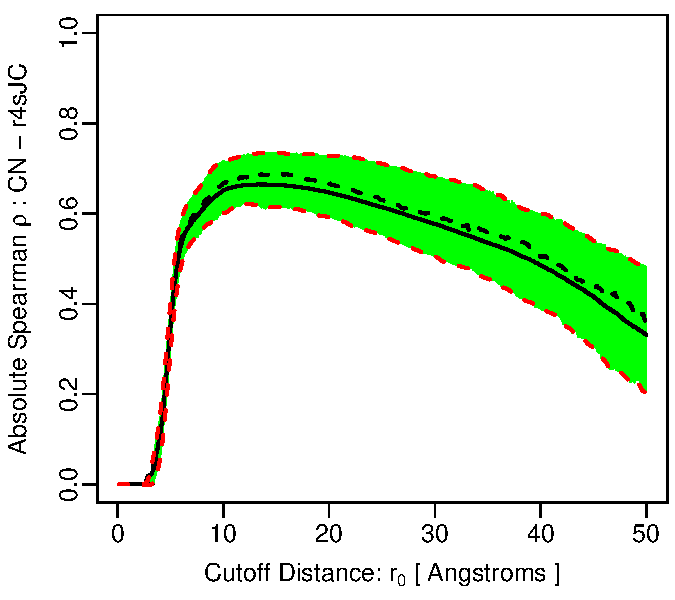
\includegraphics[width=3.3in]{../../wcn_best_definition/analysis/figures/get_quantiles/screen_plots/spcor_cnSC_r4sJC.pdf} & 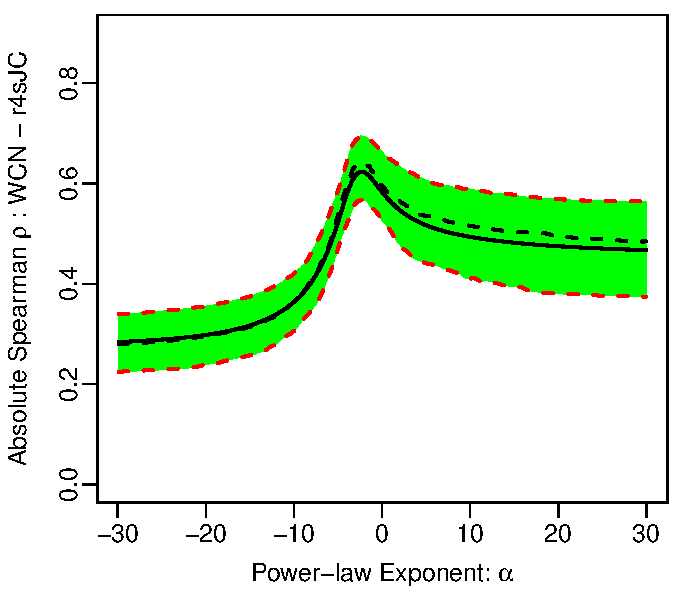
\includegraphics[width=3.3in]{../../wcn_best_definition/analysis/figures/get_quantiles/screen_plots/spcor_wcnpSC_r4sJC.pdf}
        \end{tabular}
        \end{center}
        \caption{Average absolute Spearman's correlation strengths of Contact Number (CN, as defined by Eqn. \ref{eqn:cn} using Heaviside kernel in Eqn. \ref{eqn:heaviside}) and the Weighted Contact Number (WCN, as defined by Eqn. \ref{eqn:wcn_pwrl} using a power-law kernel) with site-specific evolutionary rates, for different values of the free parameters of the two kernels ($r_0$ \& $\alpha$ respectively). On each plot, the solid black lines represent the mean correlation strength in the entire dataset of 209 proteins at each value of the free parameter, and the dashed black lines indicate the median of the distribution. The green-shaded region together with the red-dashed lines represent the $25\%$ \& $75\%$ quartiles of the correlation strength distribution. Note that for the case of WCN with $\alpha>0$ the sign of the correlation strength $\rho$ is the opposite of the sign of $\rho$ with $\alpha<0$. In addition $\rho$ is undefined at $\alpha=0$ and not shown in this plot.  The parameter values at which the Spearman's correlation coefficient reaches the maximum over the entire dataset are given in Table \ref{tab:best_params}.}
        \label{fig:cnwcnp}
    \end{figure}

    \begin{figure}
        \begin{center}
        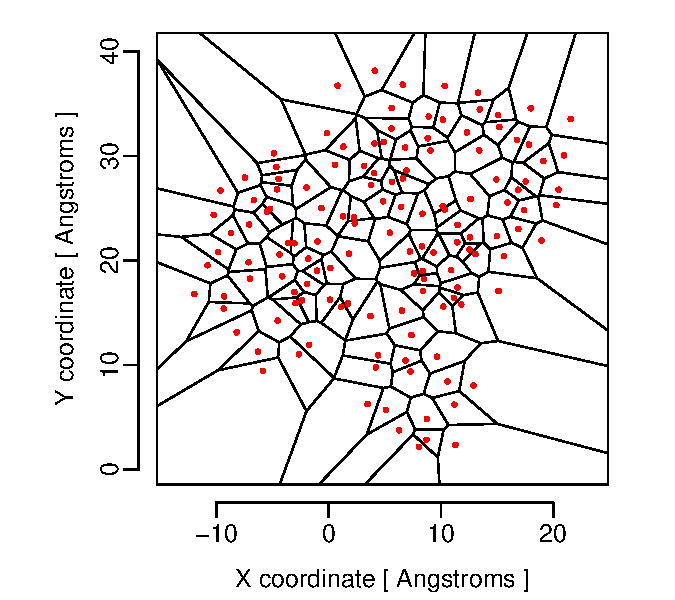
\includegraphics[width=6in]{voronoi_diagram.pdf}
        \end{center}
        \caption{An Example 2-dimensional Voronoi diagram for bacteriophage T7 lysozyme (Protein Data Bank ID `1LBA'). The red dots represent the backbone $C_\alpha$ atoms projected on the X--Y plane, used as cell seeds in Voronoi tessellation.}
        \label{fig:voronoi}
    \end{figure}

    \begin{figure}
        \begin{center}
        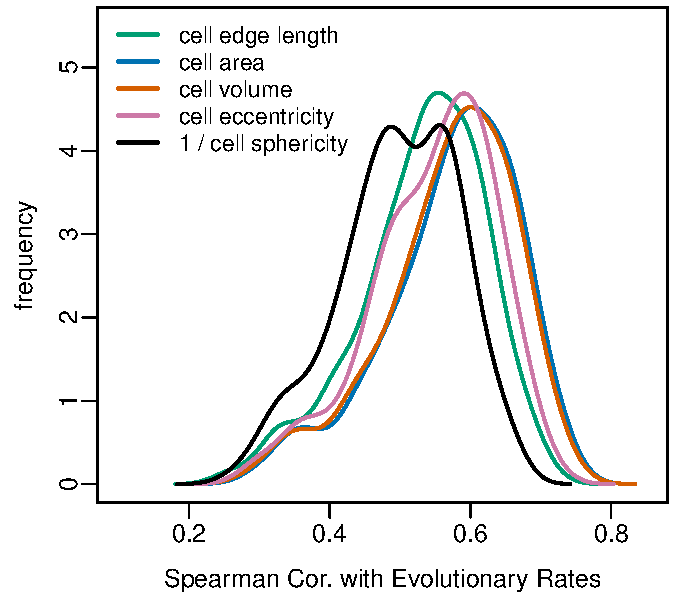
\includegraphics[width=5.5in]{best_voronoi_predictors_of_ER.pdf}
        \end{center}
        \caption{ A comparison of the prediction power of different Voronoi cell characteristics about site-specific evolutionary rates (ER). Note that all cell characteristic correlate positively with ER, except sphericity which strongly negatively correlates with ER.}
        \label{fig:voronoi_ER}
    \end{figure}

    \begin{figure}
        \begin{center}
        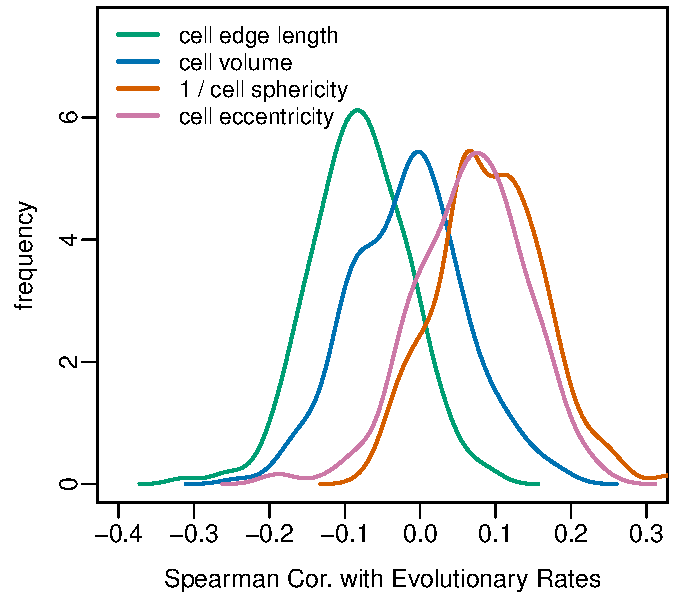
\includegraphics[width=5.5in]{best_voronoi_predictors_of_ER_given_area.pdf}
        \end{center}
        \caption{The partial correlation strengths of the same Voronoi cell characteristics with sequence evolutionary rates while controlling for the cell area.}
        \label{fig:voronoi_ER_cond}
    \end{figure}

    \begin{figure}
        \begin{center}
        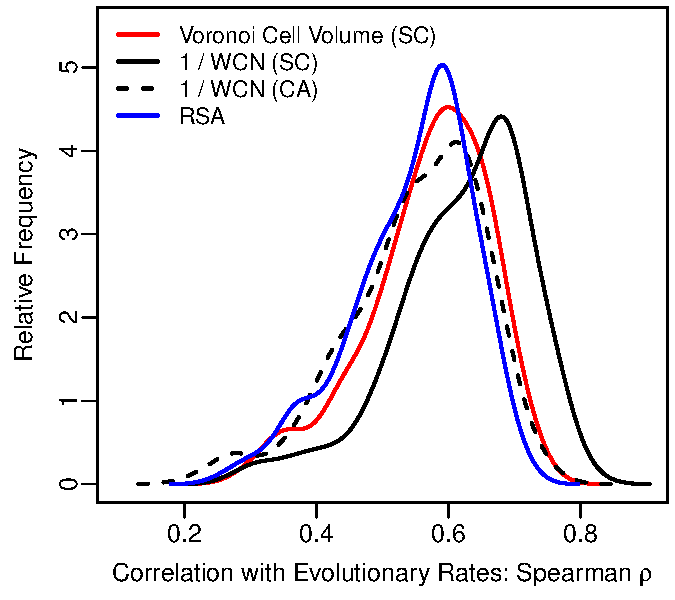
\includegraphics[width=5.5in]{best_structural_predictors_of_ER_limited.pdf}
        \end{center}
        \caption{A comparison of the prediction power of five structural variables about site-specific evolutionary rates (ER). All structural quantities correlate positively with ER, with the exception of Weighted Contact Number (WCN) which correlates negatively. For better illustration however, the Spearman's correlation coefficient ($\rho$) of the inverse of WCN with ER are shown in the Figure. Note that the Spearman's $\rho$ is a rank correlation coefficient, meaning that the use of inverse WCN only changes the sign and not the magnitude of $\rho$. The abbreviation {\it SC} refers to the use of average Side-Chain coordinates wherever used, and {\it CA} refers to the use of backbone C$_\alpha$ atomic coordinates for representation of individual sites in proteins.}
        \label{fig:best_predictorER}
    \end{figure}


    \begin{figure}
        \begin{center}
        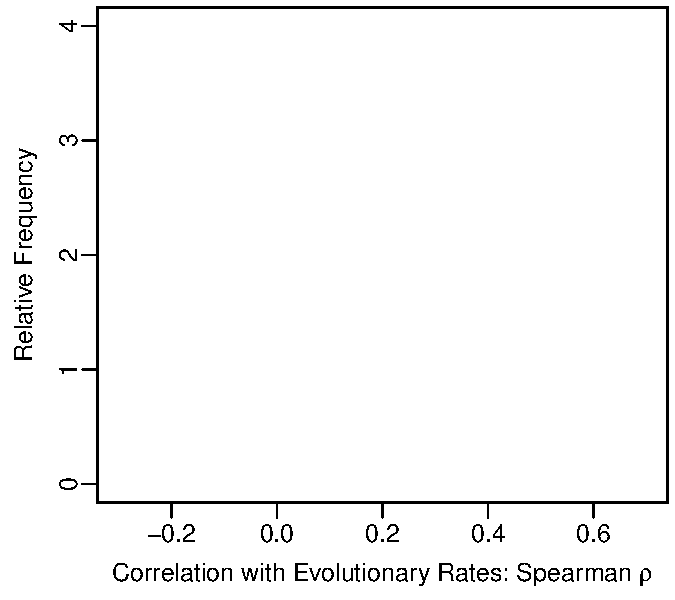
\includegraphics[width=5.5in]{best_structural_predictors_of_ER_given_vol.pdf}
        \end{center}
        \caption{A comparison of the prediction power of four structural variables (as in Figure \ref{fig:best_predictorER}) about site-specific evolutionary rates (ER), while controlling for the voronoi cell volume. All structural quantities correlate positively with ER on average, with the exception of Weighted Contact Number (WCN) which correlates negatively. For better illustration however, the Spearman's correlation coefficient ($\rho$) of the inverse of WCN with ER are shown in the Figure. Note that the Spearman's $\rho$ is insensitive to the use of inverse WCN in place of WCN. The abbreviation {\it SC} refers to the use of average Side-Chain coordinates wherever used, and {\it CA} refers to the use of backbone C$_\alpha$ atomic coordinates for representation of individual sites in proteins.}
        \label{fig:best_predictorER_given_volume}
    \end{figure}

    \begin{figure}
        \begin{center}
        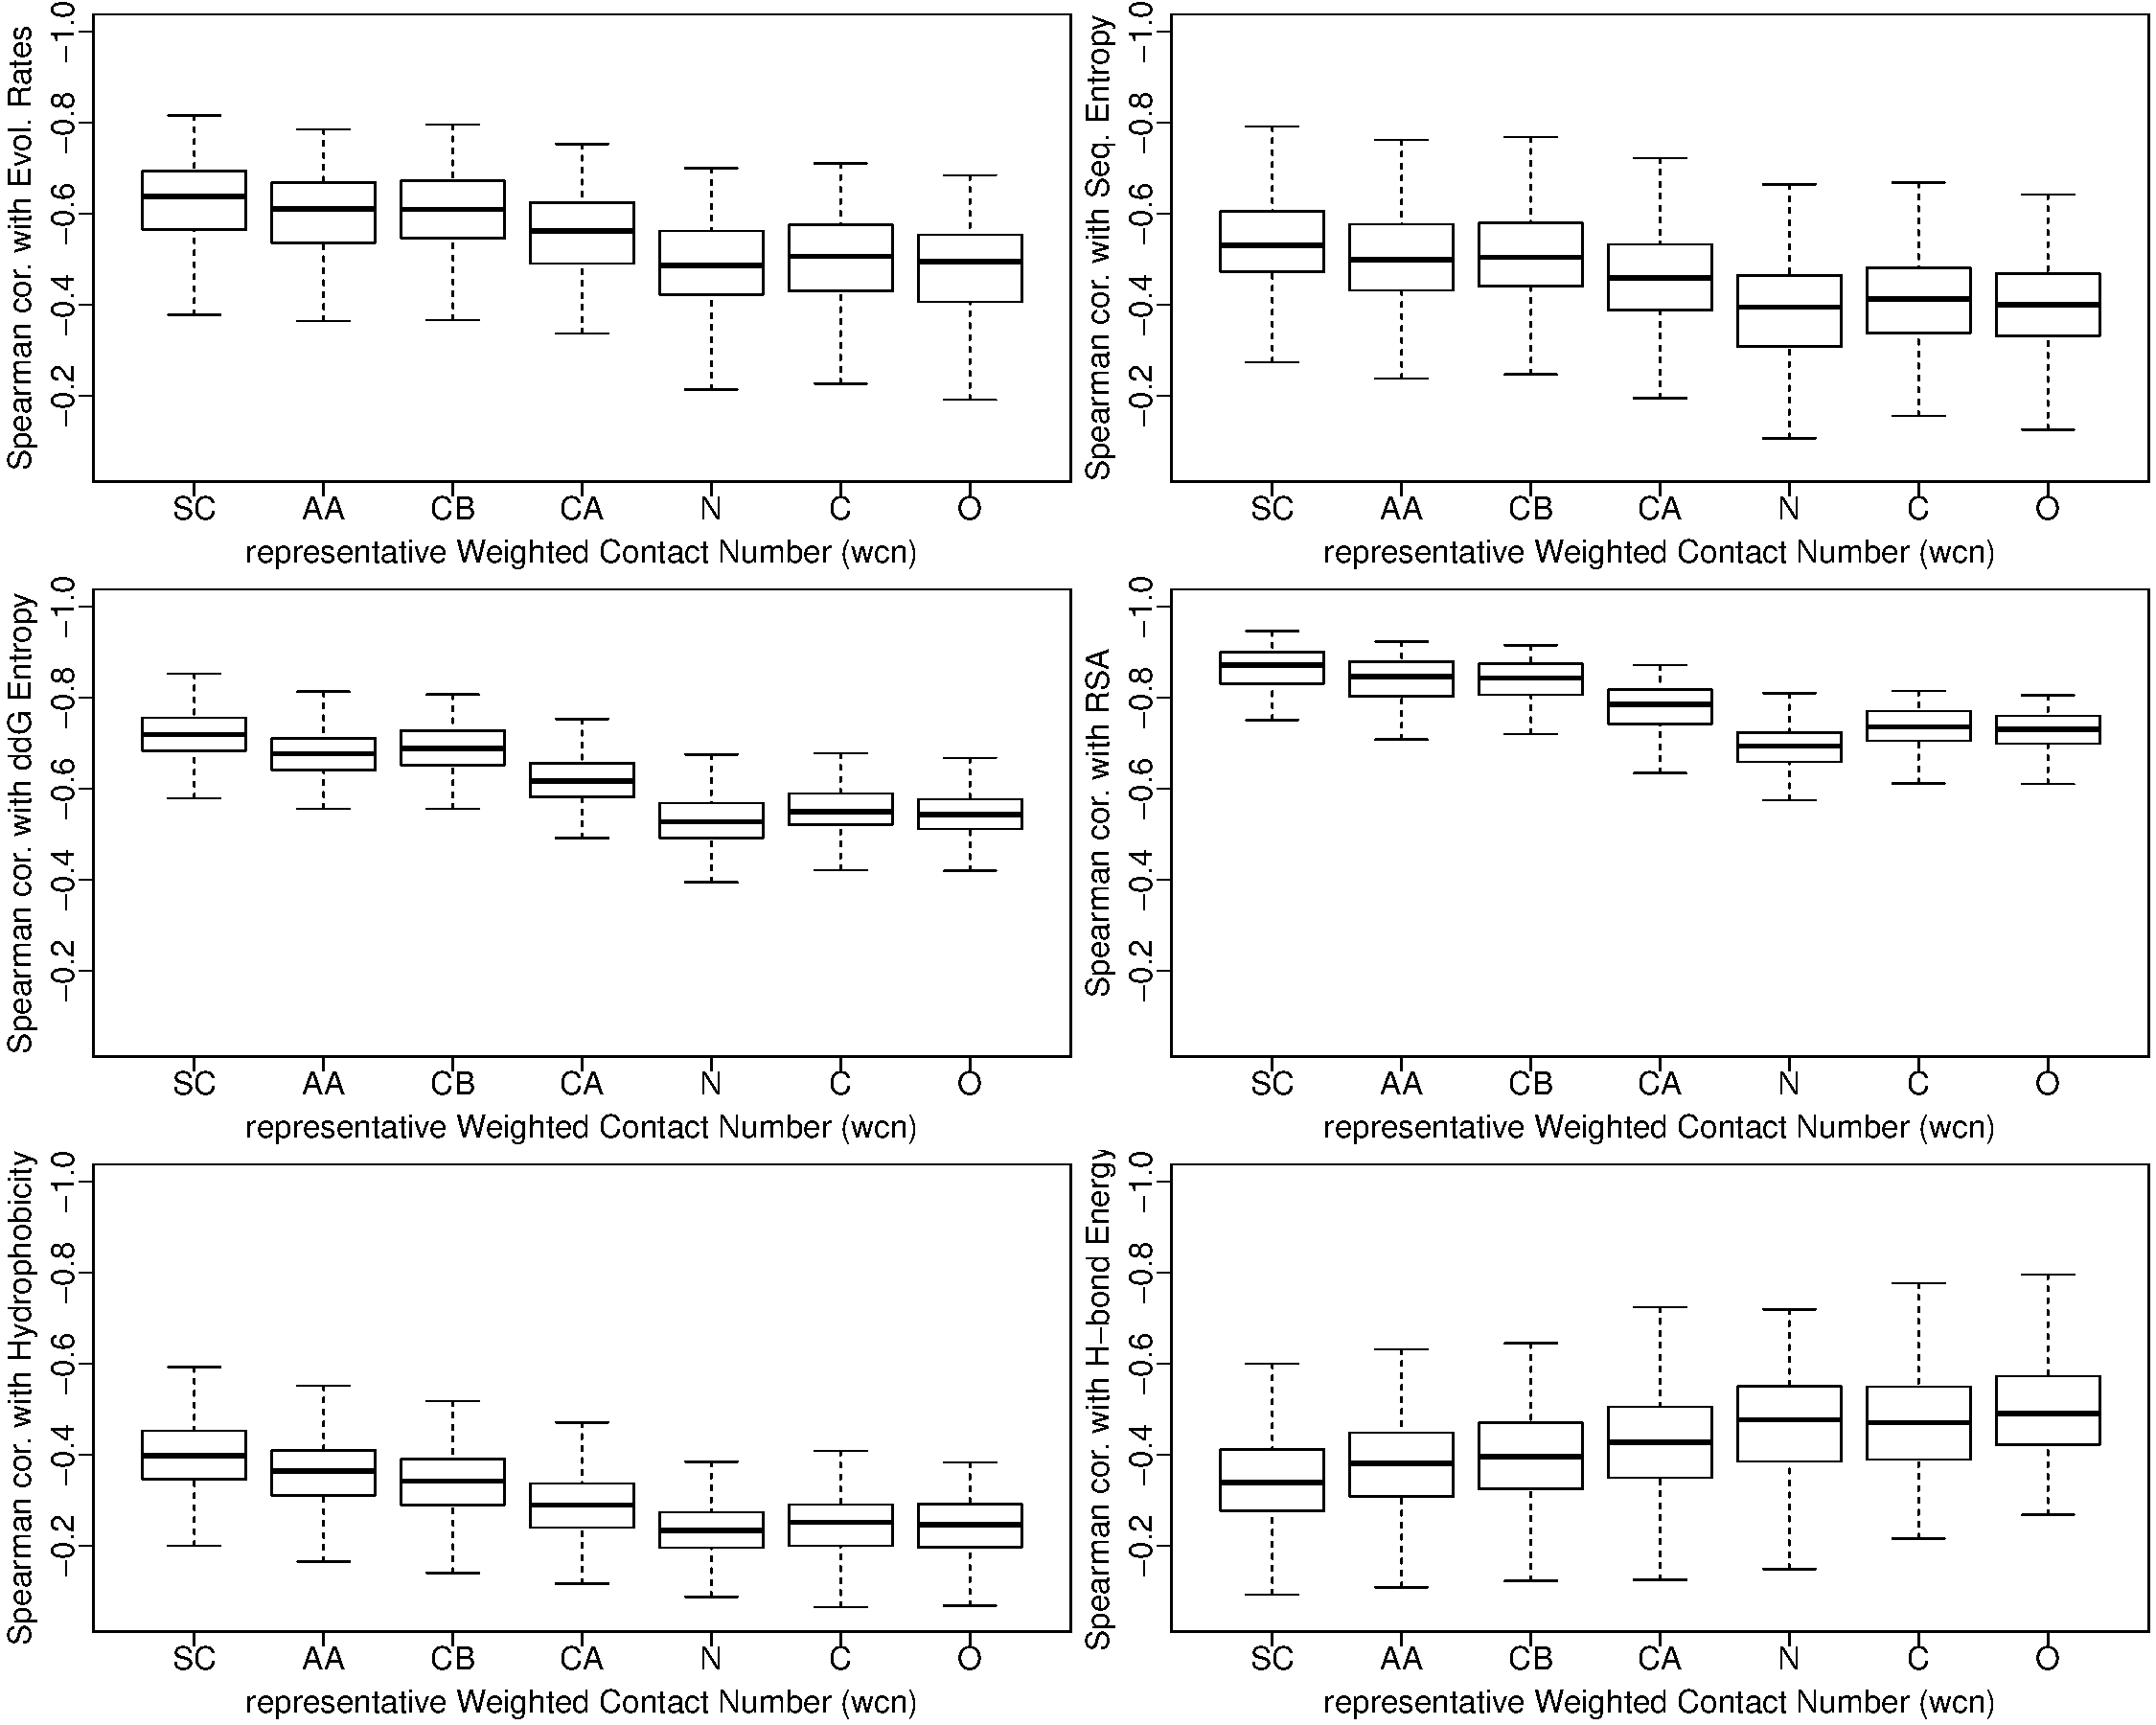
\includegraphics[width=5.5in]{best_wcn/select_variables/boxplot_wcn_all_in_one.pdf}
        \end{center}
        \caption{A comparison of the correlation strength of 6 different measures of Weighted Contact Number (WCN) with 6 coordinate-independent structural or sequence properties for 209 proteins in dataset. The contact numbers, WCN, are calculated using 6 sets of atomic coordinates: {\it SC, AA, CB, CA, N, C, O}, used as different representations of individual sites in proteins. The two labels {\it SC} \& {\it AA} stand respectively for the geometric average coordinates of the Side Chain (SC) atoms and the entire Amino Acid (AA) atoms, excluding hydrogens.}
        \label{fig:best_wcn}
    \end{figure}

    \begin{figure}
        \begin{center}
        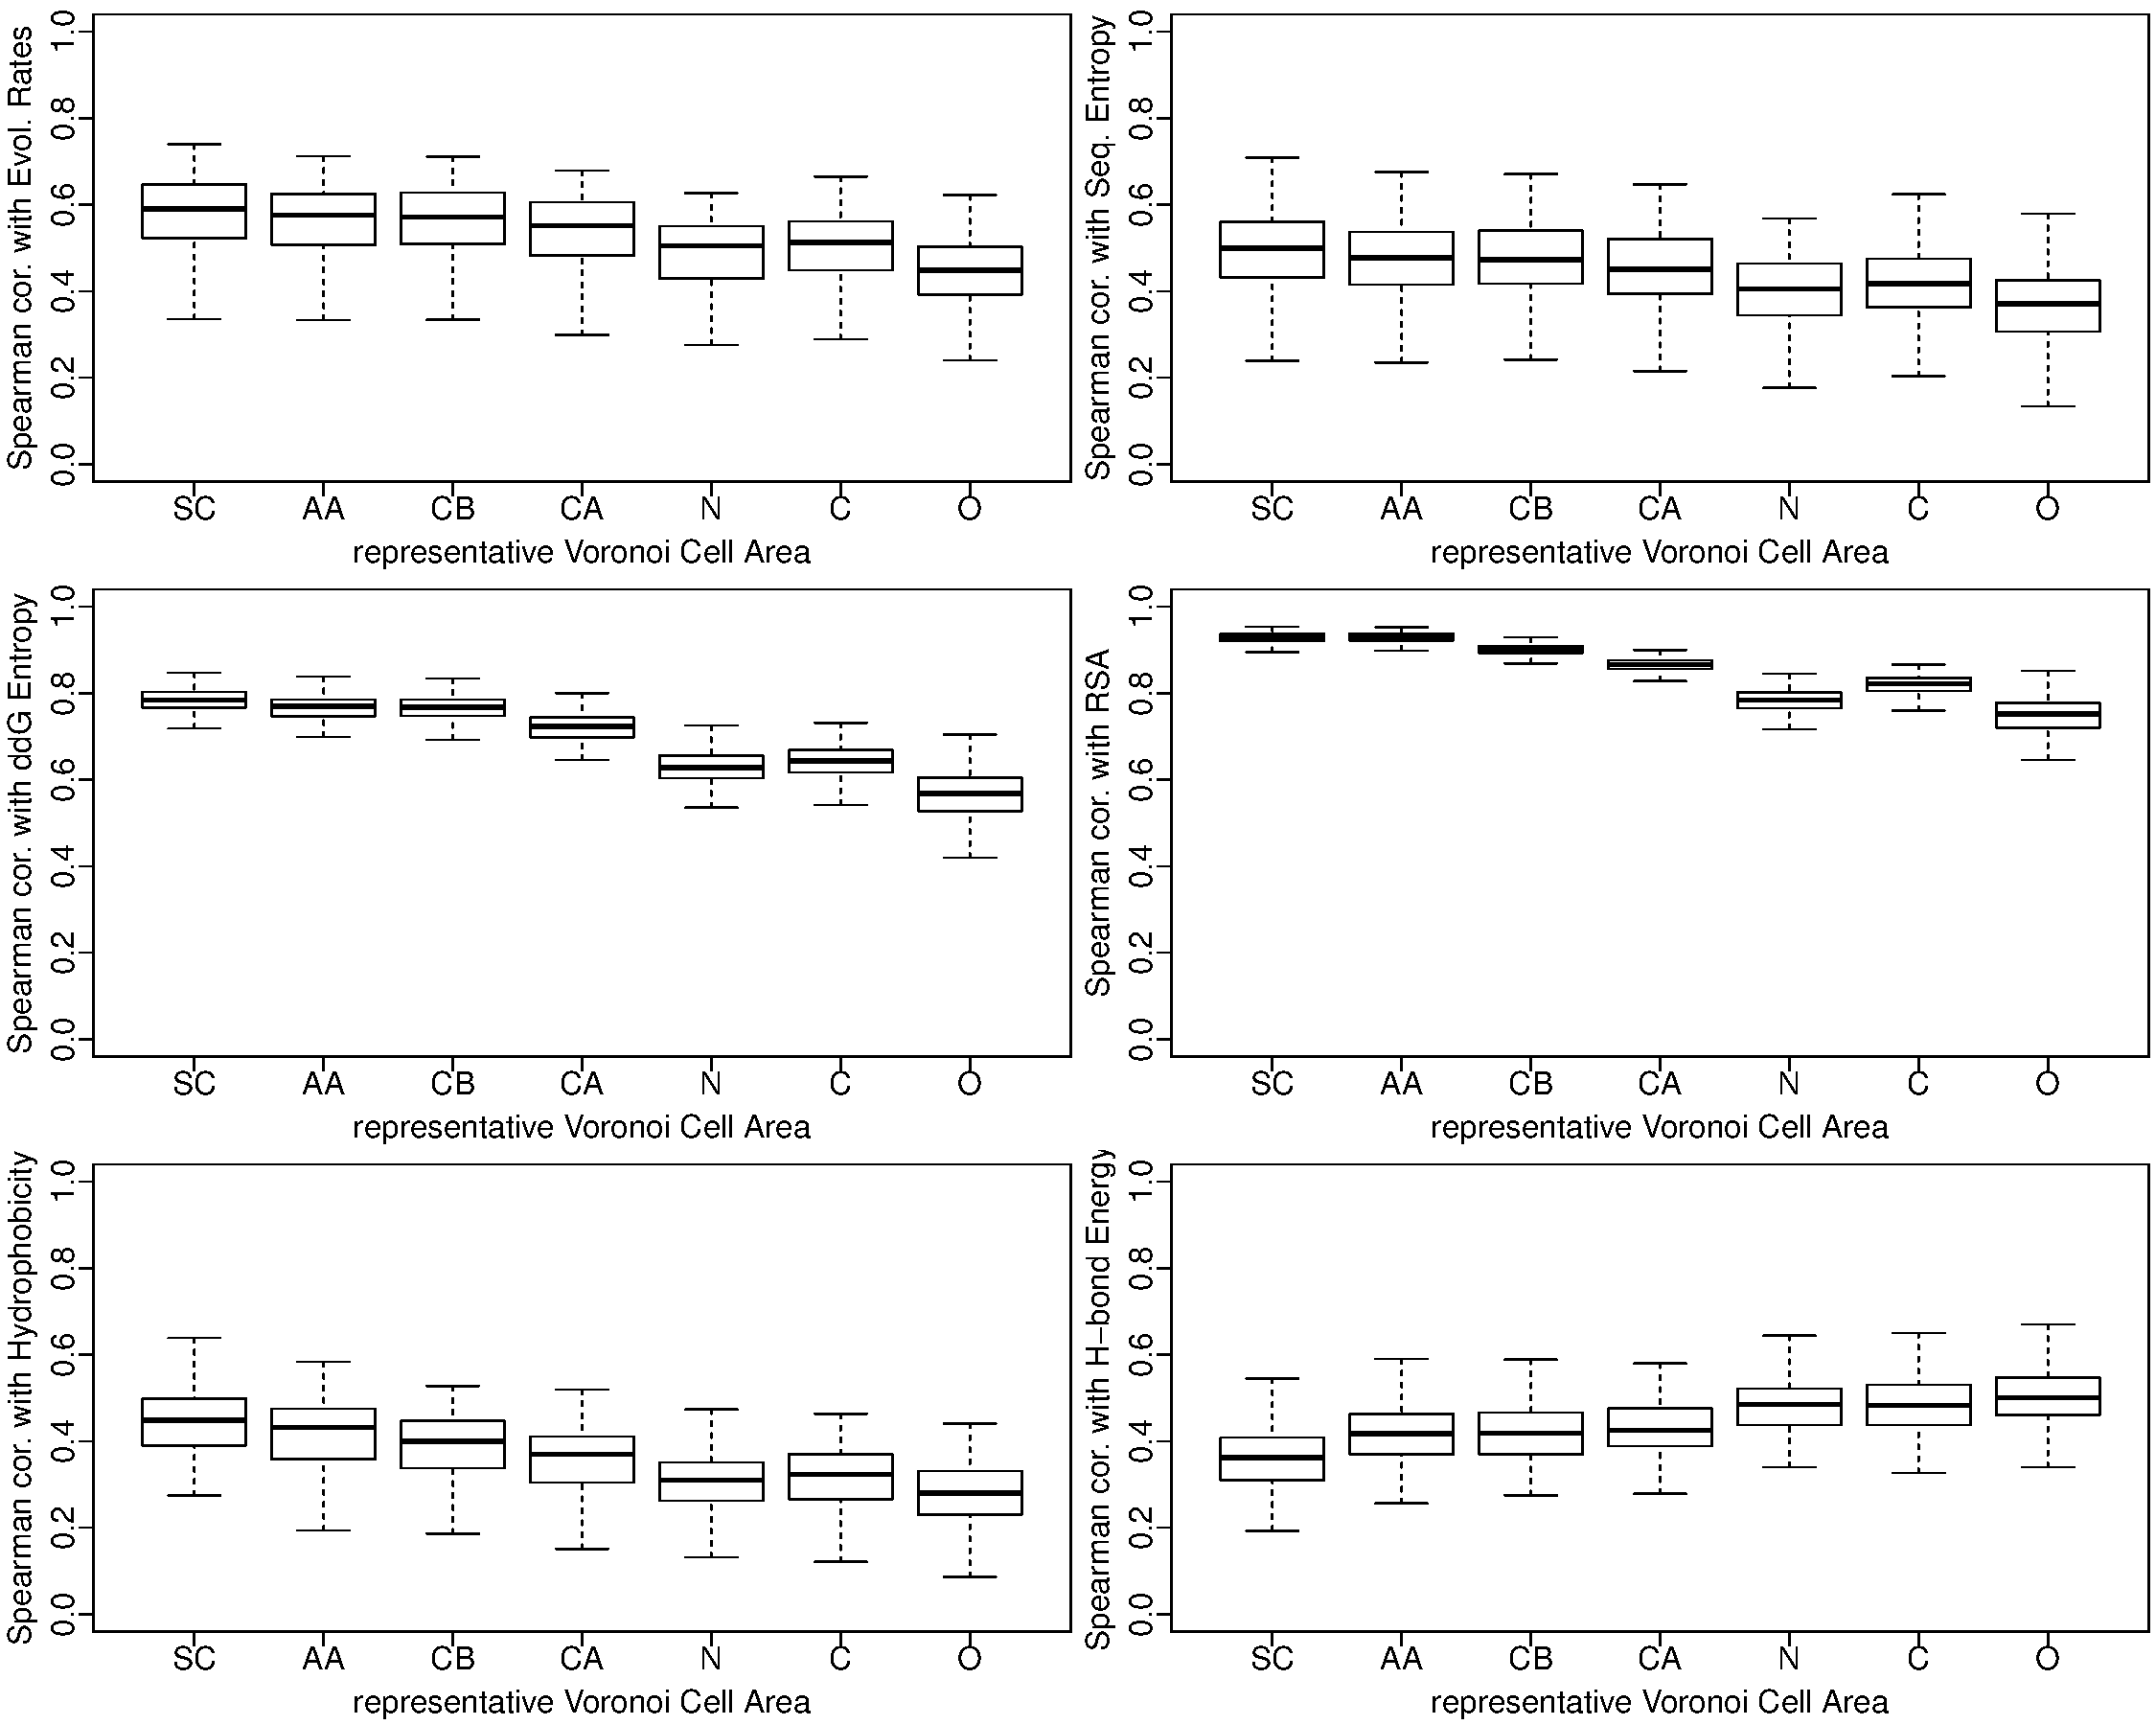
\includegraphics[width=5.5in]{best_varea/select_variables/boxplot_varea_all_in_one.pdf}
        \end{center}
        \caption{A comparison of the correlation strength of 6 different measures of Voronoi cell areas with 6 coordinate-independent structural or sequence properties for 209 proteins in dataset.  The Voronoi cells are generated using 6 sets of atomic coordinates: {\it SC, AA, CB, CA, N, C, O}, used as different representations of individual sites in proteins. The two labels {\it SC} \& {\it AA} stand respectively for the geometric average coordinates of the Side Chain (SC) atoms and the entire Amino Acid (AA) atoms, excluding hydrogens.}
        \label{fig:best_voronoi}
    \end{figure}

%    \begin{figure}
%        \begin{center}
%        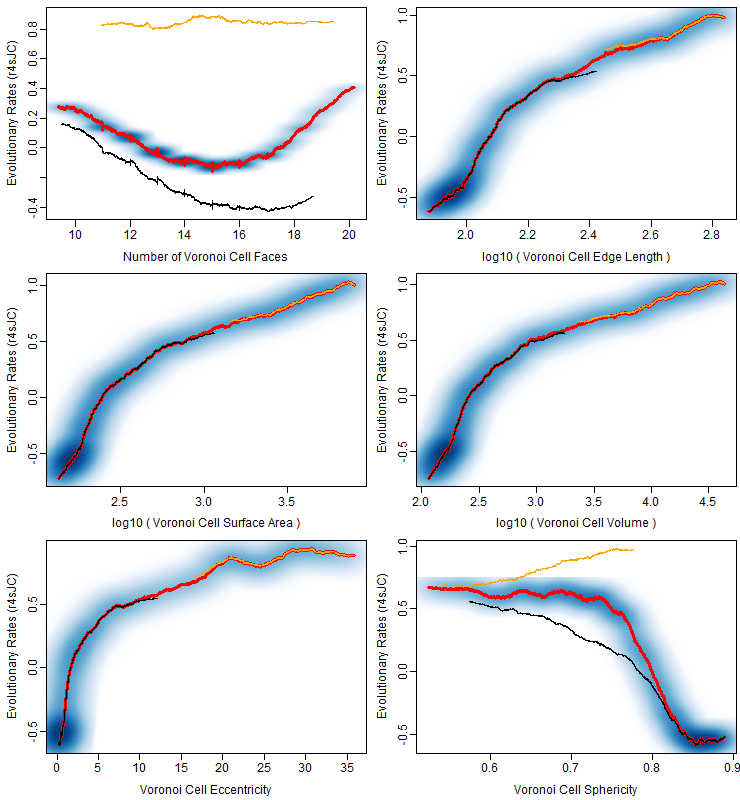
\includegraphics[width=5.5in]{adjacent_averaging_screen/only_voro/zr4s_JC_voro.png}
%        \end{center}
%        \caption{General behavior of Voronoi cell characteristics versus normalized site-specific evolutionary rates among all sites in all 209 proteins in dataset. The red curves in each plot is obtained by adjacent-averaging of every $3000$ sites. The black \& orange curves represent respectively the general behaviors of closed \& open Voronoi cell characteristics. The background heat map in each plot is a 2D density plot of all 75755 amino acid sites in all 209 proteins, showing the overall distribution of sites about the average curve.}
%        \label{fig:zr4s_JC_voro}
%    \end{figure}
%
%    \begin{figure}
%        \begin{center}
%        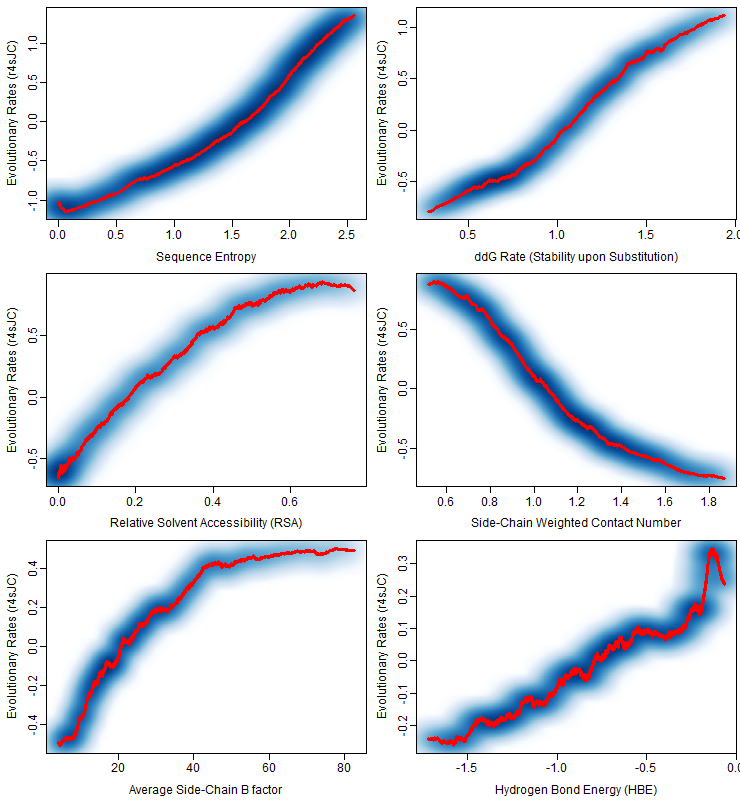
\includegraphics[width=5.5in]{adjacent_averaging_screen/only_nonvoro/zr4s_JC_nonvoro.png}
%        \end{center}
%        \caption{General behavior of site-specific structural characteristics versus normalized site-specific evolutionary rates among all sites in all 209 proteins in dataset. The red curves in each plot is obtained by adjacent-averaging of every $3000$ sites. The background heat map in each plot is a 2D density plot of all 75755 amino acid sites in all 209 proteins, showing the overall distribution of sites about the average curve.}
%        \label{fig:zr4s_JC_nonvoro}
%    \end{figure}

%    \begin{figure}
%        \begin{center}
%        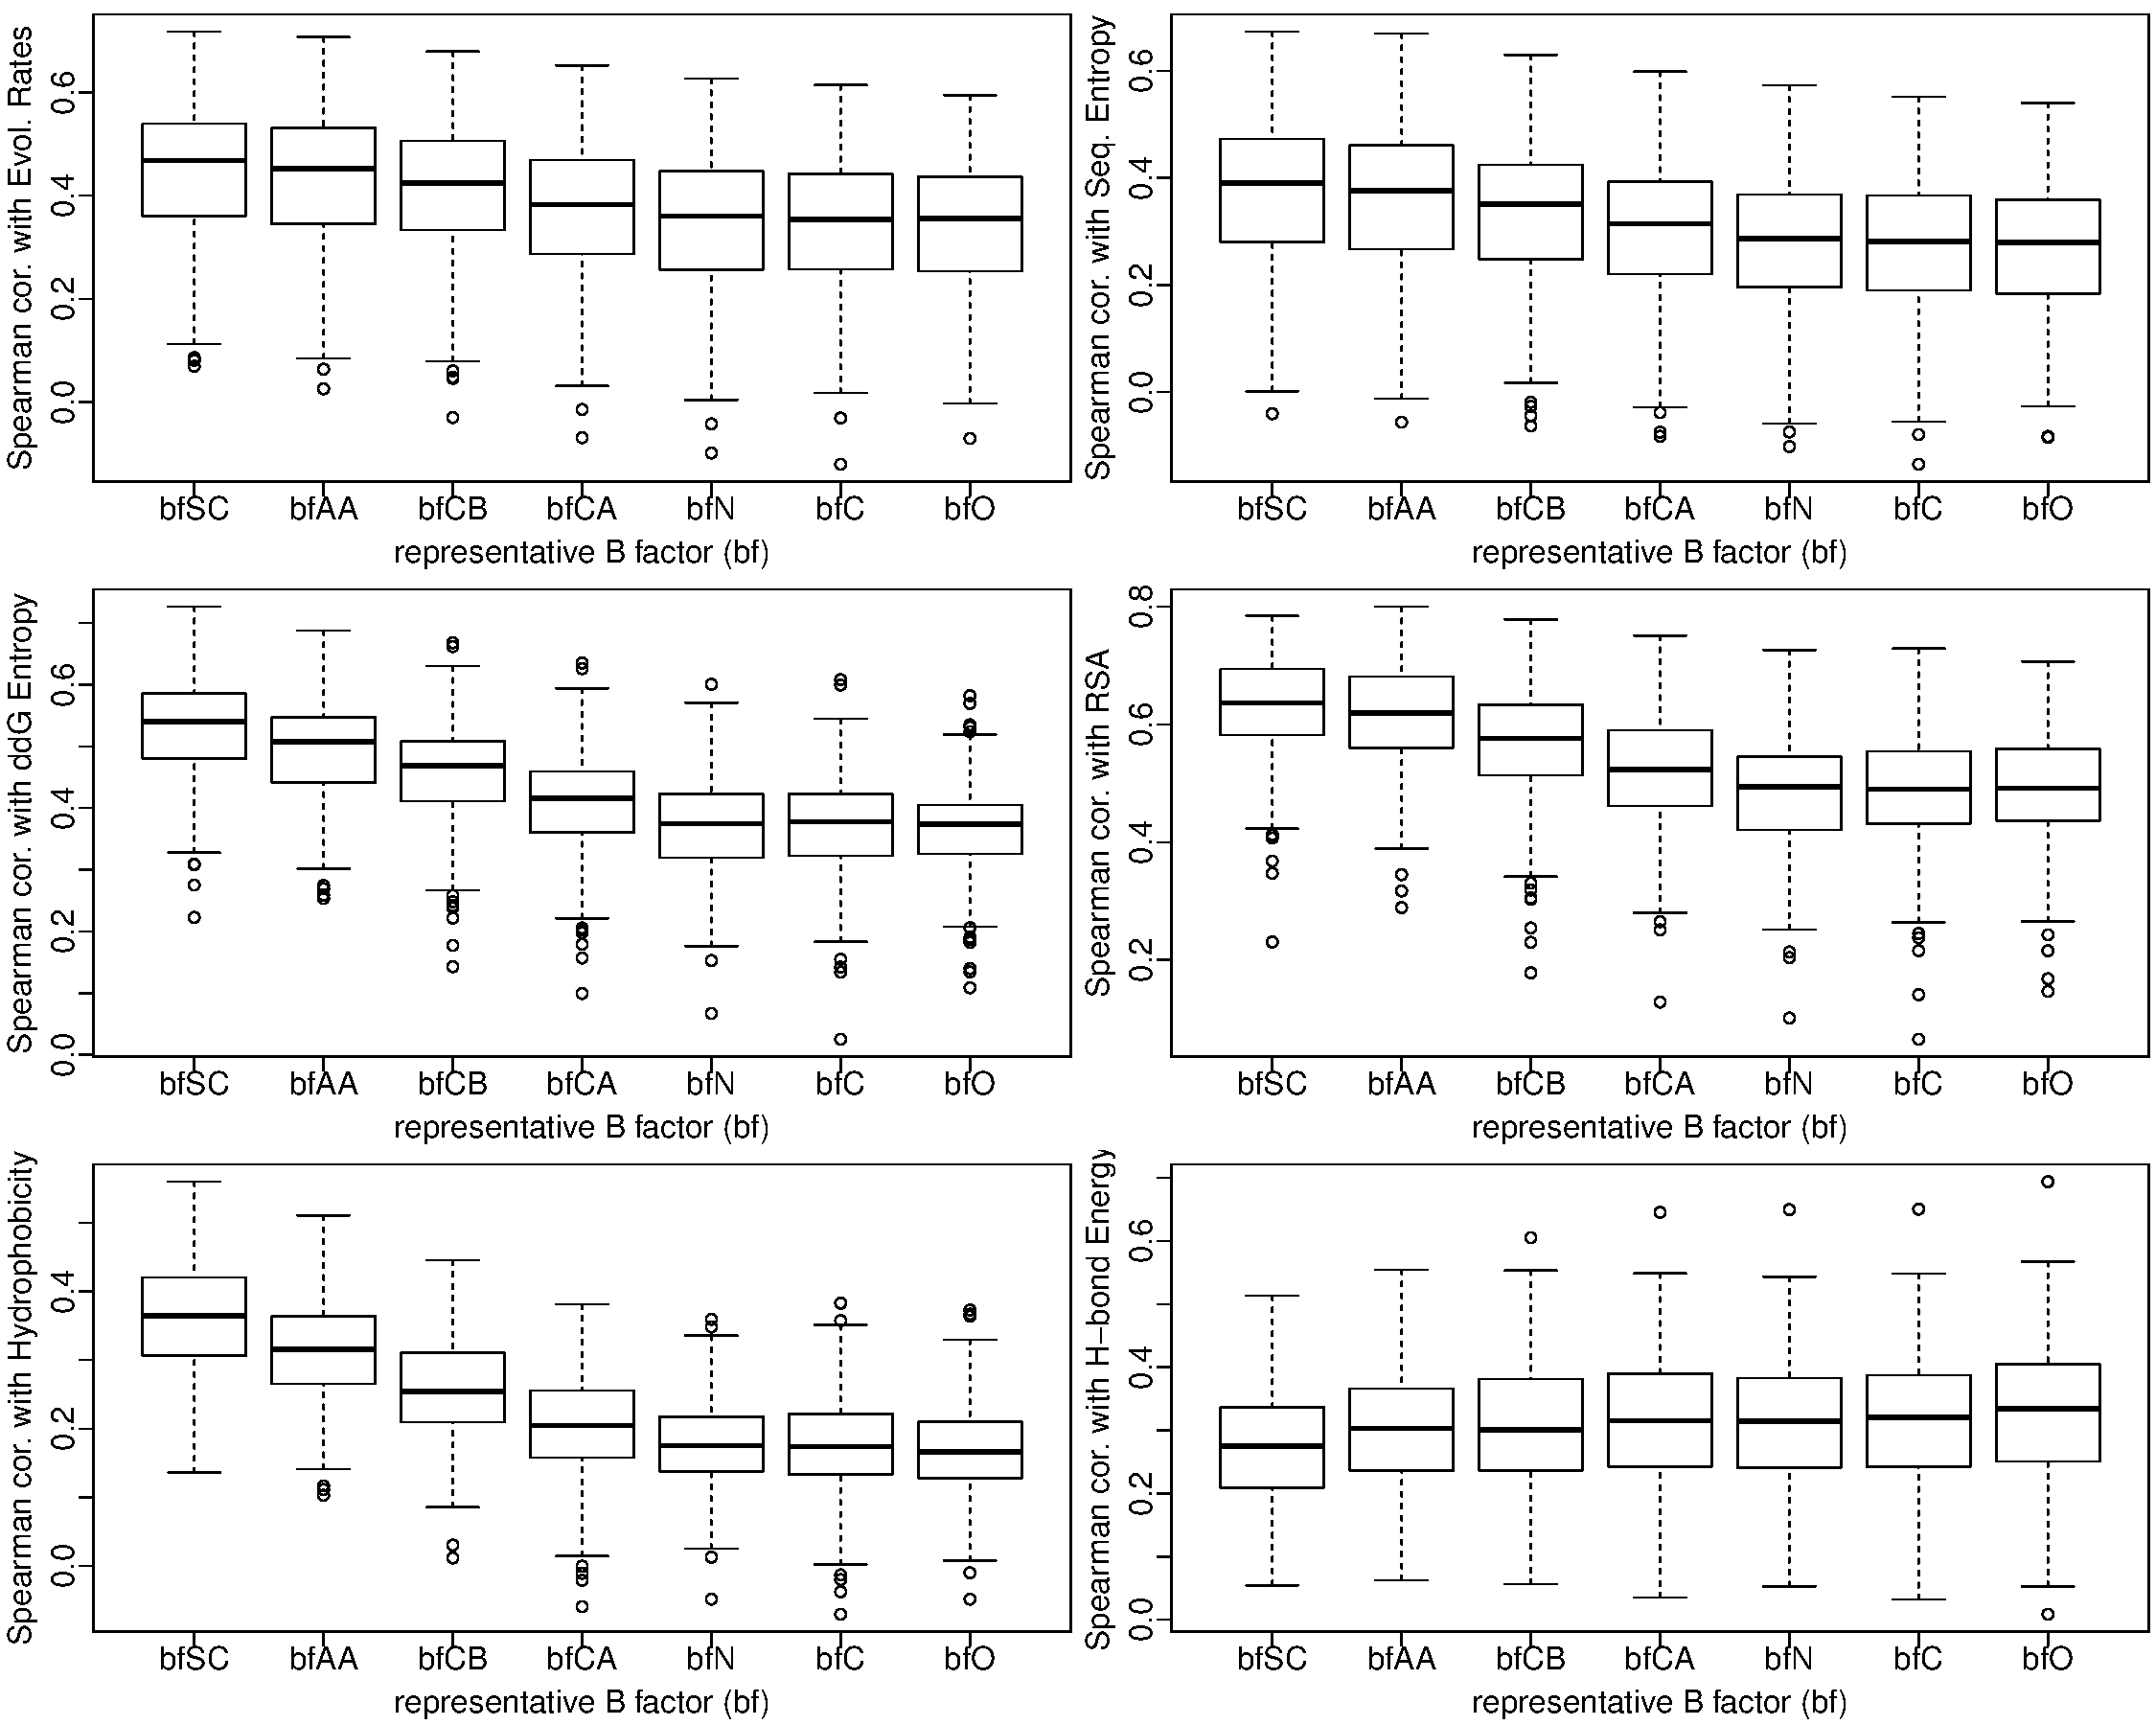
\includegraphics[width=5.5in]{best_bf/select_variables/boxplot_bf_all_in_one.pdf}
%        \end{center}
%        \caption{A comparison of the correlation strength of 6 different measures of B factor with 6 coordinate-independent structural or sequence properties for 209 proteins in dataset. Shown on the horizontal axes, are the 6 representative atomic B factors: {\it SC, AA, CB, CA, N, C, O} used as flexibility measures of individual sites in proteins. The two variables {\it SC} \& {\it AA} stand respectively for the average B factor of all Side Chain (SC) atoms and the entire Amino Acid (AA) atoms, excluding hydrogens.}
%        \label{fig:best_bf}
%    \end{figure}
%
%    \begin{figure}
%        \begin{center}
%        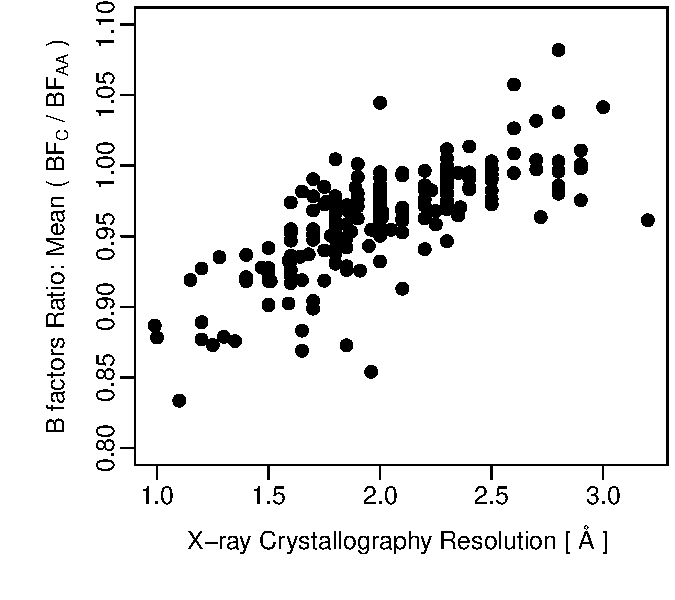
\includegraphics[width=5.5in]{mean_bfC_bfAA_ratio_resol.pdf}
%        \end{center}
%        \caption{An illustration of the strong positive correlation of X-ray crystallography resolution with the ratio of the backbone $C$ atomic B factor to the average amino acid B factor ($\text{BF}_C/\text{BF}_{AA}$), averaged over all sites in individual proteins, highlighting the significant contributions of noise and model errors to atomic B factor values. The Spearman's correlation coefficient between the two quantities is $\rho\sim0.76$. No significant correlation would be expected in the absence of noise due to limited resolution of the X-ray crystallography of proteins. Each filled circle in the plot represents one protein in the dataset of 209 enzymes used in this work.}
%        \label{fig:bfC_bfAA_ratio}
%    \end{figure}


%    \begin{figure}
%        \begin{center}
%        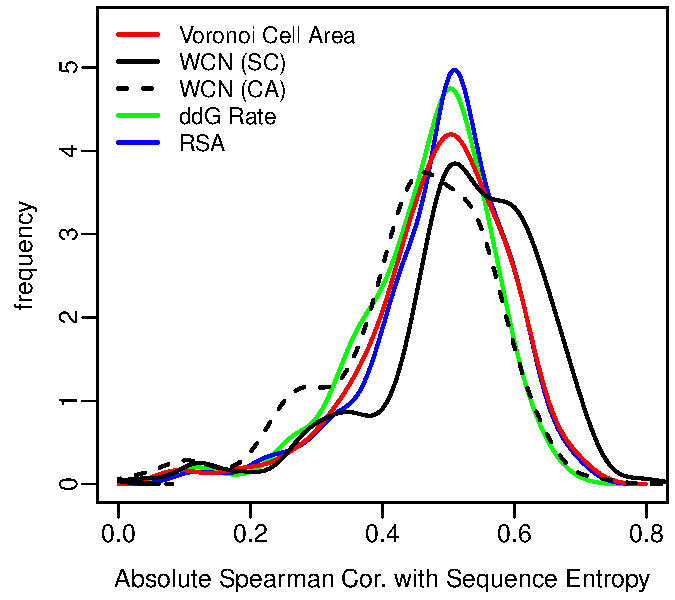
\includegraphics[width=5.5in]{best_structural_predictors_of_SE.pdf}
%        \end{center}
%          \caption{A comparison of the prediction power of five structural variables about site-specific Sequence Entropy (SE). All structural quantities correlate positively with SE, with the exception of Weighted Contact Number (WCN) which correlates negatively. For better illustration however, the Spearman's correlation coefficient ($\rho$) of the inverse of WCN with ER are shown in the Figure. Note that the Spearman's $\rho$ is a rank correlation coefficient, meaning that the use of inverse WCN only changes the sign and not the magnitude of $\rho$. The abbreviation {\it SC} refers to the use of average Side-Chain coordinates or average Side-Chain B factor wherever used, and {\it CA} refers to the use of backbone C$_\alpha$ atomic coordinates for representation of individual sites in proteins.}
%        \label{fig:best_predictorSE}
%    \end{figure}

%    \begin{figure}
%        \begin{center}
%        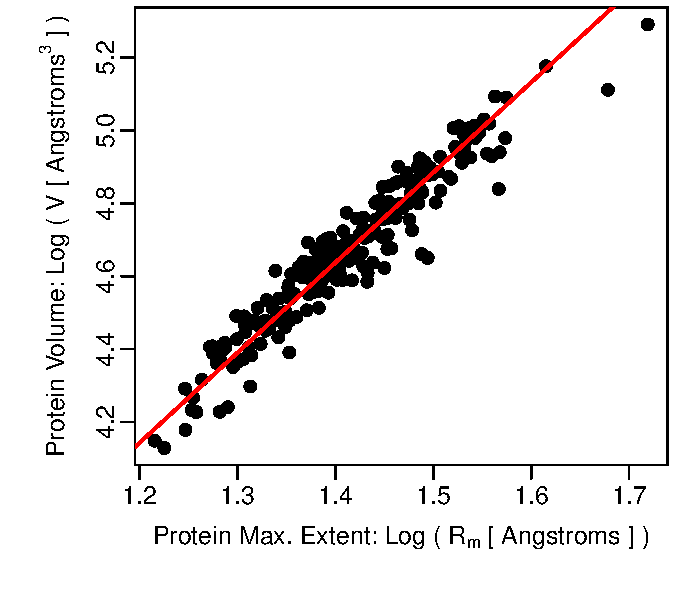
\includegraphics[width=5.5in]{fractal_dim_max_extent_volume.pdf}
%        \end{center}
%        \caption{The scaling behavior of protein maximum extent as defined by Eqn. \ref{eqn:max_extent} with protein volume for $209$ monomeric enzymes in the dataset. The red line is the linear Deming regression fit to logarithms of the two variables with a slope of $D\simeq2.47\pm0.06$.}
%        \label{fig:maxextent}
%    \end{figure}
%
%    \begin{figure}
%        \begin{center}
%        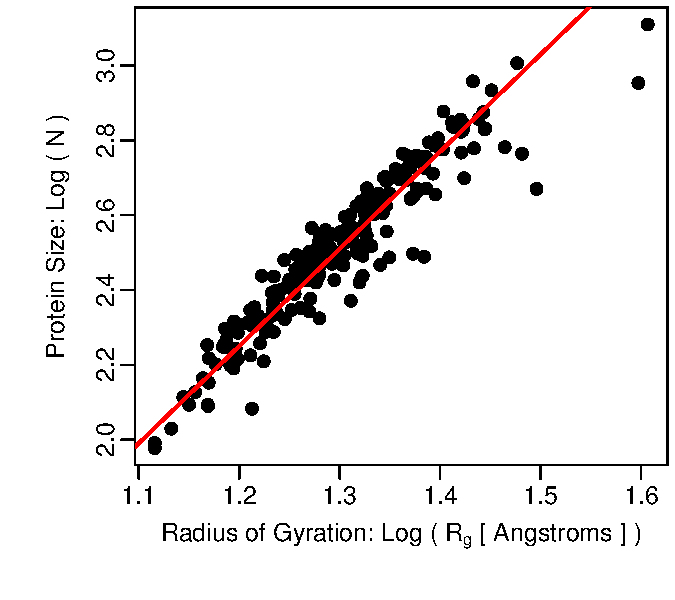
\includegraphics[width=5.5in]{fractal_dim_rad_gyration_nres.pdf}
%        \end{center}
%        \caption{The scaling behavior of protein's radius  as defined by Eqn. \ref{eqn:rg} with protein length for $209$ monomeric enzymes in the dataset. The mean \& median length of the proteins are $362$ \& $315$ respectively. The red line is the linear Deming regression fit to logarithms of the two variables with a slope of $D\simeq2.60\pm0.08$.}
%        \label{fig:rg}
%    \end{figure}


\newpage

% Tables

    \begin{table}[htbp]
    \caption{Median best free parameter values of the Contact Number (CN) and the Weighted Contact Number with power-law kernel (WCN) that result in the strongest median Spearman's correlation ($\rho$) of CN \& WCN with site-specific sequence variability measures (evolutionary rates (r4sJC) and sequence entropy) in the entire dataset of 209 proteins. Given in parentheses are the corresponding median Spearman correlation coefficients at the best parameter values. The subscripts and superscripts to each value represent the $25\%$ percentile range below and above the median value of the distribution. \label{tab:best_params}}
    \bigskip
    \centerline{
    \begin{tabular}{|l|c|c|}
      \hline
      Correlation with  & $r_0[\AA]$ (CN)      & $\alpha$ (WCN)        \\ \hline
      r4sJC             & $14.3^{+5.3}_{-4.0}$ ($\rho\sim0.64^{+0.06}_{-0.06}$) & $-2.3^{+0.8}_{-0.4}$ ($\rho\sim0.65^{+0.05}_{-0.07}$)  \\
      Seq. Entropy      & $12.4^{+5.5}_{-2.6}$ ($\rho\sim0.55^{+0.06}_{-0.06}$) & $-2.2^{+0.8}_{-0.4}$ ($\rho\sim0.55^{+0.07}_{-0.06}$)  \\
      %B factor          & $13.1^{+4.0}_{-2.2}$ ($\rho\sim0.70^{+0.05}_{-0.06}$) & $-2.2^{+0.5}_{-0.4}$ ($\rho\sim0.71^{+0.05}_{-0.06}$)  \\
      \hline
    \end{tabular}}
    \end{table}

    \begin{table}[htbp]
    \caption{The percentage of variance of site-specific evolutionary rates (r4sJC) explained by site-specific packing density (represented by the inverse volume of Voronoi cells) and long-range amino acid interactions (as described in Sec. \ref{sec:long_range}). For each structural quantity, the first, second (median) and the third quartiles of the percentage distribution of the explained variance are reported on each row, for the entire dataset of 209 proteins.  \label{tab:best_params}}
    \bigskip
    \centerline{
    \begin{tabular}{|l|c|c|c}
      \hline
      \multirow{2}{*}{structural quantity} & variance explained ($25\%$ quartile) & variance explained (median) & variance explained ($75\%$ quartile)  \\ \hline
      site-specific packing density      & $27\%$ & $34\%$ & $41\%$  \\
      long-range amino-acid interactions & $5\%$  & $10\%$ & $16\%$  \\
      \hline
    \end{tabular}}
    \end{table}

\end{document}

